\newcommand{\DoNotLoadEpstopdf}{}
\documentclass[11pt]{article}
\usepackage[T1]{fontenc}
\usepackage[utf8]{inputenc}
\usepackage{lmodern}
\usepackage[margin=1in]{geometry}
\usepackage{microtype}
\usepackage{amsmath,amssymb,amsthm,mathtools}
\usepackage{enumitem,booktabs,array}
\usepackage{tikz,tikz-cd}
\usetikzlibrary{arrows.meta,positioning,calc,fit,backgrounds}
\usepackage[numbers,sort&compress]{natbib}
\PassOptionsToPackage{hyphens}{url}
\usepackage[colorlinks=true,linkcolor=blue!55!black,citecolor=blue!55!black,urlcolor=blue!55!black]{hyperref}
\usepackage[capitalise,noabbrev]{cleveref}
\hypersetup{pdftitle={Thomason Model Structures in Every Strict Higher Dimension},pdfauthor={OpenAI}}
\ifdefined\pdfinfoomitdate\pdfinfoomitdate=1\fi
\ifdefined\pdftrailerid\pdftrailerid{}\fi
\ifdefined\pdfsuppressptexinfo\pdfsuppressptexinfo=15\fi
\pdfglyphtounicode{parenleftbig}{0028 FE01}
\pdfglyphtounicode{parenrightbig}{0029 FE01}
\pdfglyphtounicode{vextendsingle}{20D3}
\pdfglyphtounicode{braceleftBigg}{007B FE04}
\pdfglyphtounicode{bracerightBigg}{007D FE04}
\pdfglyphtounicode{bracelefttp}{23A7}
\pdfglyphtounicode{braceleftbt}{23A9}
\pdfglyphtounicode{braceleftmid}{23A8}
\pdfglyphtounicode{summationdisplay}{2211 FE02}
\pdfglyphtounicode{coproductdisplay}{2210 FE02}
\pdfglyphtounicode{hatwide}{02C6 FE01}
\pdfglyphtounicode{hatwider}{02C6 FE02}
\pdfglyphtounicode{tildewide}{02DC FE01}
\pdfglyphtounicode{arrowhookleft}{21AA}
\pdfglyphtounicode{mapsto}{21A6}
\setlength{\emergencystretch}{2em}
\numberwithin{equation}{section}
\newtheorem{theorem}{Theorem}[section]
\newtheorem{lemma}[theorem]{Lemma}
\newtheorem{proposition}[theorem]{Proposition}
\newtheorem{corollary}[theorem]{Corollary}
\theoremstyle{definition}
\newtheorem{definition}[theorem]{Definition}
\newtheorem{example}[theorem]{Example}
\theoremstyle{remark}
\newtheorem{remark}[theorem]{Remark}
\newcommand{\nCat}{n\mathrm{Cat}}
\newcommand{\omCat}{\omega\mathrm{Cat}}
\newcommand{\sSet}{\mathrm{sSet}}
\newcommand{\Street}{N_n}
\newcommand{\OrdN}{N}
\newcommand{\U}[1]{U_{#1}}
\newcommand{\Uinf}[1]{U^{\infty}_{#1}}
\newcommand{\Disk}[1]{D_{#1}}
\newcommand{\Orient}[1]{\mathcal O_{#1}}
\newcommand{\trunc}{\tau_n}
\newcommand{\Sd}{\mathrm{Sd}}
\newcommand{\Ex}{\mathrm{Ex}}
\newcommand{\id}{\mathrm{id}}
\DeclareMathOperator{\Hom}{Hom}
\DeclareMathOperator*{\colim}{colim}
\DeclareMathOperator{\Ob}{Ob}
\DeclareMathOperator{\im}{im}
\DeclareMathOperator{\sk}{sk}
\DeclareMathOperator{\dom}{dom}
\DeclareMathOperator{\cod}{cod}
\newcommand{\KQ}{\mathrm{KQ}}
\newcommand{\inj}{\text{-}\mathrm{inj}}
\newcommand{\cell}{\text{-}\mathrm{cell}}
\newcommand{\cof}{\text{-}\mathrm{cof}}
\title{Thomason Model Structures in Every Strict Higher Dimension}
\author{OpenAI}
\date{September 25, 2026}
\begin{document}
\maketitle
\begin{abstract}
We prove the higher-dimensional Thomason model-structure conjecture of
Ara and Maltsiniotis. For every $1\le n\le\infty$, the category of small
strict globular $n$-categories admits a proper combinatorial model structure
that is Quillen equivalent to simplicial sets. Its weak equivalences and
fibrations are detected by the twice-extended Street nerve $\Ex^2N_n$, and
the Quillen equivalence is given by $c_n\Sd^2\dashv\Ex^2N_n$. Thus strict
higher categories model the homotopy theory of spaces in every positive
finite dimension and in dimension $\omega$.
\end{abstract}
\tableofcontents
\section{Introduction}
\label{sec:introduction}

Thomason's model structure equips the category of small categories with
the homotopy theory of spaces. Its higher-dimensional analogue asks for
the same result on the entire category of strict globular
$n$-categories, with weak equivalences detected by the Street nerve and
fibrations detected by its twice-extended nerve. We prove this analogue
in every dimension, resolving positively the higher-dimensional
Thomason model-structure conjecture of Ara and Maltsiniotis.

Fix a universe of small sets and enlarge the universe when forming
categories of small objects. For a positive integer $n$, let $\nCat$ be
the category of small strict globular $n$-categories and strict functors.
We regard it as the full subcategory of $\omCat$ consisting of strict
$\omega$-categories whose cells above dimension $n$ are identities; for
$n=\infty$, set $\nCat=\omCat$. There is no invertibility assumption on
positive-dimensional cells.
The Street nerve and its left adjoint are denoted by
\[
 c_n:\sSet\rightleftarrows\nCat:N_n,
 \qquad (N_nX)_m=\Hom_{\omCat}(\Orient{m},X),
\]
where $\Orient{m}$ is the $m$th oriental. With the usual subdivision
adjunction $\Sd\dashv\Ex$, put
\[
 L_n=c_n\Sd^2,\qquad R_n=\Ex^2N_n.
\]
Write $W_{\KQ}$ and $\mathrm{Fib}_{\KQ}$ for the weak homotopy
equivalences and Kan fibrations of simplicial sets, and define
\begin{equation}
\label{eq:prescribed-classes}
 W_n=R_n^{-1}(W_{\KQ})=N_n^{-1}(W_{\KQ}),\qquad
 F_n=R_n^{-1}(\mathrm{Fib}_{\KQ}),\qquad
 C_n={}^{\perp}(F_n\cap W_n).
\end{equation}
Here ${}^{\perp}$ denotes the left lifting class. The equality defining
$W_n$ follows from the classical properties of $\Ex$, recalled in
Section~\ref{sec:transfer}.

\begin{theorem}\label{thm:main}
For every $n\in\{1,2,3,\ldots\}\cup\{\infty\}$, the classes
$(C_n,W_n,F_n)$ in \eqref{eq:prescribed-classes} form a proper
combinatorial model structure on $\nCat$. It is cofibrantly generated by
$(L_nI,L_nJ)$, where
\[
 I=\{\partial\Delta[m]\hookrightarrow\Delta[m]:m\ge0\},\qquad
 J=\{\Lambda^k[m]\hookrightarrow\Delta[m]:m\ge1,\ 0\le k\le m\}.
\]
Moreover,
\[
 L_n:\sSet_{\KQ}\rightleftarrows(\nCat,C_n,W_n,F_n):R_n
\]
is a Quillen equivalence.
\end{theorem}

\subsection*{History and significance}
Thomason established the case $n=1$ by transferring the simplicial
model structure through $c_1\Sd^2\dashv\Ex^2N_1$
\cite{Thomason1980}. His proof separates two issues that persist in
higher dimensions: the homotopy behavior of the adjunction unit and
the comparison between a pushout of nerves and the nerve of a
categorical pushout. For the latter he introduced Dwyer maps and proved
the comparison for their arbitrary cobase changes
\cite[Definition~4.1 and Proposition~4.3]{Thomason1980}.
Cisinski corrected the retract argument used for properness, while
preserving the model structure and its properness
\cite{Cisinski1999}.
Street's orientals extend the nerve to strict higher categories
\cite{Street1987}, providing the weak equivalences in the question
considered here.

Ara and Maltsiniotis developed an abstract transfer theorem, drawing
on the homotopy theory of categories developed by Grothendieck and
Cisinski, and established the proper combinatorial model structure
in dimension two. Using Chiche's comparison theorem for the
homotopy categories of categories and $2$-categories, they also
obtained the Quillen equivalence
\cite[Theorems~4.11, 6.27, 6.30, and Corollary~6.32]{AraMaltsiniotis2014}.
Worytkiewicz, Hess, Parent, and Tonks had proposed the two-dimensional
structure earlier \cite{WorytkiewiczHessParentTonks2007}; their later
corrigendum addresses the gaps identified by Ara and Maltsiniotis
\cite{WorytkiewiczHessParentTonks2016}.
For arbitrary $1\le n\le\infty$, the transfer framework isolates two
sufficient conditions: a unit comparison on nerves of posets, and
preservation of certain poset equivalences by every categorical
pushout \cite[Scholie~5.14]{AraMaltsiniotis2014}.

Ara and Maltsiniotis proved the poset-unit condition in all these
dimensions \cite[Corollary~10.11 and Scholie~10.12]{AraMaltsiniotis2015}.
Gagna subsequently gave a direct simplicial proof and showed that
the Street nerve induces an equivalence with homotopy types after
localizing at the nerve weak equivalences
\cite[Theorems~5.6 and~6.9]{Gagna2018}.
Thus strict higher categories already described the homotopy category
of spaces in every dimension. The prescribed model structure requires
the additional lifting and factorization statements, whose construction
depends on controlling actual categorical pushouts. Ara's 2023 account
records this remaining sufficient condition and the general conjecture
\cite[\S\S9.2.5--9.2.6]{Ara2023}; Guetta and Maltsiniotis also state
the $\omega$-dimensional model-structure conjecture explicitly
\cite[Introduction, p.~6]{GuettaMaltsiniotis2024}.

The shapes of higher cells matter in this question. Fiore and Paoli
constructed a Thomason model structure on small $n$-fold categories,
whose weak equivalences are detected by the diagonal of the $n$-fold
nerve and which is Quillen equivalent to simplicial sets
\cite[Theorem~9.28]{FiorePaoli2010}.
Their objects are obtained by iterating the internal-category
construction; the present theorem concerns strict globular categories
and the Street nerve.

Theorem~\ref{thm:main} supplies both weak factorization systems on all
strict $n$-categories, together with left and right properness, by
establishing the remaining pushout condition. Its arbitrary-target
scope is essential: the small object argument must allow attachments
to categories that need not be cofibrant or freely generated.
The $\omega$-dimensional proof uses finite orientals directly, and
finite-dimensional reflection carries the same construction to each
finite $n$.

\subsection*{Stationary cylinders and the pushout argument}
For a poset $E$, write $\U{E}=c_n\OrdN E$, where $\OrdN$ is the ordinary
nerve. The principal intermediate result is
Theorem~\ref{thm:couniversal}: if $A\subseteq E$ is a downward-closed
full subposet and its inclusion has a right adjoint retraction, then
every pushout of $\U{A}\to\U{E}$ is a Street weak equivalence.
This proves the sufficient condition isolated in
\cite[Scholie~5.14, condition~(d$'$)]{AraMaltsiniotis2014}.
The cylinders used for contraction fix $\U{A}$ throughout the interval.
After any attachment $\U{A}\to X$, this equality lets each
cylinder glue to the constant cylinder on $X$, controlling the entire
pushout and its newly formed composites.

The construction starts with a restricted but explicit directed prism.
Suppose $f,g:E\to E$ are monotone, $f\le g$, they agree on a sieve $A$,
and $g$ is constant on $E\setminus A$. Write $u$ for the degree-one
generator of the interval chain complex. For every increasing tuple $w$,
the formula
\[
 [w_0,\ldots,w_p]\otimes u
 \longmapsto [fw_0,\ldots,fw_p,gw_p]
\]
together with the endpoint maps induced by $f$ and $g$ defines a positive
chain map after normalized repetitions are set to zero. It produces a
strict Gray cylinder constant in the interval direction on $\U{A}$,
at the common endpoint restriction induced by $f|_A=g|_A$.
Its positivity is a consequence of the precise hypotheses on the old
part and the constant upper map. Section~\ref{sec:prisms} proves the
chain identity, compatibility with all simplex operators, and descent
to every finite dimension.

When $E\setminus A$ has a greatest element, we choose two such
cylinders whose defining poset maps restrict to $\id_A$.
They give a relative contraction by a zigzag, which extends across
any attachment. For a general finite poset, deleting
distinct maximal new elements gives two sieves containing $A$.
The corresponding pushouts are full sieve subcategories of the total
attachment, with intersection the pushout for the common subposet.
Their nerves form an ordinary pushout along
monomorphisms, so the local weak-equivalence statements glue. This
allows each local contraction to be chosen independently. Finite
subposets stable under the retraction then yield the result for
arbitrary posets.

The remaining comparison follows the geometry of Thomason's Dwyer
maps \cite[Propositions~4.2--4.3]{Thomason1980}.
Two subdivisions put each generating boundary or horn inclusion into
the form $\OrdN A\hookrightarrow\OrdN B$, where $A$ is a sieve and
its inclusion into its upward closure in $B$ has a right adjoint
retraction (Lemma~\ref{lem:subdivision-posets}). For any small poset
pair with these properties, Proposition~\ref{prop:attachment-comparison}
provides a reusable comparison between the pushout of Street nerves
and the nerve of an attachment along an arbitrary functor $\U{A}\to X$.
The poset description here concerns the generating pieces.

At the chain level we use Steiner's description of orientals
\cite{Steiner2004,Steiner2007} and the biclosed Gray tensor product,
with the completed extension theorem of Ara and Maltsiniotis
\cite[Theorem~A.15]{AraMaltsiniotis2020}.
Positive-chain constructions already give simplicial nerve homotopies
in Gagna's proof \cite[Sections~6.3--6.8]{Gagna2018}.
Here the restricted prism hypotheses give strict relative cylinders;
the choices fixing $A$ extend across arbitrary attachments.
The cover calculations build on the
fiber and sieve machinery of Ara and Maltsiniotis
\cite[Lemma~2.8 and Propositions~5.3 and~5.5]{AraMaltsiniotis2014};
they allow us to glue the weak-equivalence conclusions without choosing
compatible contractions on overlapping pieces.

\subsection*{Organization}
Section~\ref{sec:foundations} records the foundations and the precise
simplicial gluing lemma. Sections~\ref{sec:prisms} and
\ref{sec:pieces} construct the stationary cylinders and identify
labelled pieces. Section~\ref{sec:couniversality} proves couniversality
and the unit comparison for posets. Section~\ref{sec:attachments}
proves the nerve comparison for subdivided boundary and horn
attachments, with explicit control of the monomorphic gluing legs.
Section~\ref{sec:transfer} supplies the model axioms, properness, and
the unit comparison for arbitrary simplicial sets.
Appendix~\ref{app:presentability} proves the required presentability
and smallness assertions by guarded term presentations.
Appendix~\ref{sec:context} discusses the relationship with the
elementary-expansion method for Grothendieck groupoids; its claims are not inputs to the
proof.

\section{Strict categories, directed chains, and simplicial gluing}
\label{sec:foundations}

The pushout argument needs three foundations: directed chain maps must
give strict right cylinders, these cylinders must descend to finite
dimensions, and their nerve comparisons must survive gluing and filtered
colimits. We fix the conventions and prove the needed local statements
before constructing the relative prism.

We work with small objects in a fixed universe.  An $\omega$-category in
this paper is a strict globular $\omega$-category: its cells have globular
sources and targets, identities, and compositions along matching
lower-dimensional boundaries, satisfying the associativity, unit, and
interchange laws strictly.  An $n$-category, for finite $n$, has only
identity cells above dimension $n$.  The inclusion
$\nCat\hookrightarrow\omCat$ has a left adjoint $\trunc$.
Explicitly, $\trunc X$ retains the cells of $X$ in dimensions below $n$,
and its $n$-cells are the $n$-cells of $X$ modulo the congruence generated
by
\[
 s_n(z)=t_n(z)\qquad(z\text{ an }(n+1)\text{-cell of }X).
\]
Here the congruence is closed under every defined composition.  Its
generating pairs are parallel $n$-cells, so their identifications leave
every lower matching boundary unchanged; compositions therefore descend
to the quotient.  Cells above $n$ become identities.  Every strict functor from $X$ to an
$n$-category annihilates these relations, which proves the stated
reflection property.  We set $\tau_\infty=\id$ and use $\nCat=\omCat$
when $n=\infty$.

Write $\Disk{i}$ for the free strict $\omega$-category on one $i$-cell,
with all its globular faces.  Thus
$\Hom_{\omCat}(\Disk{i},X)$ is the set of $i$-cells of $X$,
$\Disk{0}$ is terminal, and $\Disk{1}$ is the category $0\to1$.
Let $\Orient{m}$ denote the $m$th oriental.  Its standard cosimplicial
structure defines
\[
 (\Street X)_m=\Hom_{\omCat}(\Orient{m},X)
              =\Hom_{\nCat}(\trunc\Orient{m},X).
\]
For $\omega$-categories we also write $N_\infty$.  The left adjoints are
given by the simplex colimits
\begin{equation}\label{eq:categorification-colimit}
 c_\infty K=\colim_{(\Delta[m]\to K)\in\Delta/K}\Orient{m},
 \qquad
 c_nK=\trunc c_\infty K
     =\colim_{(\Delta[m]\to K)\in\Delta/K}\trunc\Orient{m}.
\end{equation}
These formulas follow from the universal property of a colimit and the
degreewise definition of the nerve.  In particular, for a poset $E$,
\[
 \Uinf{E}=c_\infty\OrdN E,\qquad
 \U{E}=c_n\OrdN E=\trunc\Uinf{E}.
\]
The fixed dimension is suppressed in $U$: for a monotone map $f$,
write $U(f)=c_n\OrdN(f)$ and $U^\infty(f)=c_\infty\OrdN(f)$.
We use $\OrdN$ for the ordinary nerve.  On ordinary categories it agrees
with the Street nerve: a map from an oriental is determined by its
successive edges, because its triangular cells impose the usual
composition equations.  In particular $N_\infty\Disk{1}=\Delta[1]$.

\subsection{The directed tensor convention}

An augmented directed complex is a nonnegative chain complex $K$ of
abelian groups, with augmentation $\epsilon:K_0\to\mathbb Z$ and a
specified additive submonoid $K_p^+\subset K_p$ in each degree.
Its morphisms are chain maps preserving the augmentation and these
submonoids.  All complexes used below have a specified free basis, with
positive submonoids generated by the basis.  For such a complex write
$dc=d^+c-d^-c$ with disjoint positive supports.  A basis is
\emph{unital} when
$\epsilon((d^-)^p b)=\epsilon((d^+)^p b)=1$ for each basis element
$b$ of degree $p$, and is \emph{strongly loop-free} when the relations
\[
 a<b\quad\text{if }a\text{ occurs in }d^-b,
 \qquad
 b<a\quad\text{if }a\text{ occurs in }d^+b
\]
are contained in a strict partial order on the whole basis.
A complex with such a basis is called a \emph{strong Steiner complex}.

Steiner's functor $\nu$ sends augmented directed complexes to strict
$\omega$-categories.  Its cells retain the lower-dimensional boundary
data of a chain.  More concretely, a $p$-cell of $\nu K$ is a table
\begin{equation}\label{eq:steiner-cell-table}
 (x_0^-,x_0^+\mid x_1^-,x_1^+\mid\cdots\mid x_p^-,x_p^+),
 \qquad x_r^\pm\in K_r^+,
\end{equation}
such that
\[
 \epsilon x_0^- = \epsilon x_0^+ = 1,\qquad
 d x_r^- = d x_r^+ = x_{r-1}^+-x_{r-1}^-
 \quad(1\le r\le p),\qquad x_p^-=x_p^+.
\]
An identity appends a zero pair to the table.  A positive,
augmentation-preserving chain map acts on every entry, giving the
corresponding strict functor
\cite[Definitions~2.6 and~2.8, Proposition~2.7]{Steiner2004}.
For a basis element $b$ of degree $p$, its \emph{atom} has top pair
$(b,b)$ and entries
$\langle b\rangle_r^\pm=(d^\pm)^{p-r}b$ for $0\le r\le p$:
at each step, take the negative or positive part of the boundary.
For a strong Steiner complex these tables are cells, and $\nu K$ is
freely generated as a polygraph by the atoms of its basis.  In
particular, maps out of it are determined by the images of these atoms
\cite[\S3 before Definition~3.2, Theorem~6.1]{Steiner2004}.
The concrete complexes needed here are as follows:
\begin{enumerate}[label=(\roman*)]
\item
The normalized simplex complex $M[m]$ has degree-$p$ basis
$[i_0,\ldots,i_p]$ for $0\le i_0<\cdots<i_p\le m$, with
\[
 d[i_0,\ldots,i_p]
   =\sum_{j=0}^{p}(-1)^j[i_0,\ldots,\widehat{i_j},\ldots,i_p]
 \quad(p>0),\qquad \epsilon[i]=1.
\]
It is strong Steiner and $\nu M[m]=\Orient{m}$.  A monotone map of
ordinals acts by applying it to the tuple; a tuple with a repeated
entry is zero.  The atom of a nonempty tuple has its first and last
vertices as its $0$-source and $0$-target.
\item
The globe complex $G[i]$ has one top basis element in degree $i$ and
two basis elements, its source and target faces, in each degree below
$i$.  Its positive-degree differentials are target minus source, and
its vertices have augmentation one.  It is strong Steiner and
$\nu G[i]=\Disk{i}$.  For $i=0$ there is just one vertex.
\end{enumerate}
The strong Steiner properties and tensor closure follow from
\cite[Examples~3.8--3.10]{Steiner2004}. The disk identification follows
from \cite[Example~4.7 and Theorem~5.11]{Steiner2004}. For the oriental
identification and its cosimplicial action, including repeated entries,
see \cite[Theorem~3.2 and \S4 before Theorem~4.1]{Steiner2007}.

The tensor of augmented directed complexes uses the ordinary
nonnegative chain-complex tensor, with separate augmentation:
\begin{equation}\label{eq:tensor-differential}
 d(x\otimes y)=dx\otimes y+(-1)^{|x|}x\otimes dy,
 \qquad
 \epsilon(x\otimes y)=\epsilon(x)\epsilon(y)
 \quad(|x|=|y|=0).
\end{equation}
Its positive submonoid is generated by the tensors of positive
elements.  Tensor products of the indicated bases are the relevant
positive bases.

We use the biclosed Gray tensor product on \emph{all} strict
$\omega$-categories supplied by
\cite[Theorem~A.15 and \S A.16]{AraMaltsiniotis2020}.
It has unit $\Disk{0}$, preserves small colimits separately in each
variable, and has canonical natural identifications
\begin{equation}\label{eq:steiner-tensor}
 \nu K\otimes\nu L\ \cong\ \nu(K\otimes L)
 \qquad(K,L\text{ strong Steiner}).
\end{equation}
Naturality here is for every morphism between strong Steiner
complexes, including maps sending basis elements to sums or zero.
This is the completed extension theorem; the general extension is
not being inferred from the incomplete proof of
\cite[Theorem~7.3]{Steiner2004}.
In particular, preservation of colimits in this paper is a property
of the Gray tensor, not a claimed preservation property of $\nu$.

It follows that $\Disk{i}\otimes\Disk{1}$ is generated by the atoms
indexed by pairs of globe basis elements, of dimension the sum of
their dimensions.  The same holds for
$\Orient{m}\otimes\Disk{1}$.  Globe face inclusions and simplex face
inclusions identify the corresponding based subcomplexes, and hence
the corresponding atoms in these tensor products.  One way to see the
last assertion directly is to compute the positive and negative
boundaries of a basis element within the based subcomplex: they are
unchanged by its inclusion.  The atom construction therefore gives
the same cell in the larger complex.

Throughout, the interval is the \emph{right} tensor factor.  Write
$e_0,e_1$ for the degree-zero basis elements of $M[1]$ and $u$ for its
degree-one element, so that $du=e_1-e_0$.  Also write
$e_a:\Disk{0}\to\Disk{1}$ for its endpoint functors and
$\epsilon:\Disk{1}\to\Disk{0}$ for the unique functor.  The projection
is
\[
 \pi_X=\id_X\otimes\epsilon:
 X\otimes\Disk{1}\longrightarrow X\otimes\Disk{0}\cong X.
\]
No interchange of the two tensor factors is used.

\subsection{Right cylinders and truncation}

Biclosedness supplies an $\omega$-category $H(Y)$ and natural
bijections
\begin{equation}\label{eq:right-internal-hom}
 \Hom_{\omCat}(X,H(Y))
   \cong\Hom_{\omCat}(X\otimes\Disk{1},Y).
\end{equation}
In the notation of \cite[\S A.18]{AraMaltsiniotis2020},
$H(Y)=\Hom_{\mathrm{oplax}}(\Disk{1},Y)$; the representing formula
\eqref{eq:right-internal-hom} fixes the convention.
Evaluation at $e_0,e_1$ and precomposition with $\pi_X$ give,
respectively, the endpoints and constant cylinders.
To extend cylinders through pushouts in $\nCat$, we will transpose
them to functors into $H(Y)$.  The next lemma shows that this
construction stays within $\nCat$ when the target $Y$ does.

\begin{lemma}[Internal hom and reflection]\label{lem:internal-truncation}
Let $n<\infty$ and let $Y$ be a strict $n$-category.  Then $H(Y)$ is a
strict $n$-category.  Consequently the reflection unit $X\to\trunc X$
induces a natural bijection
\begin{equation}\label{eq:truncated-cylinder-bijection}
 \Hom_{\omCat}((\trunc X)\otimes\Disk{1},Y)
 \ \xrightarrow{\ \cong\ }\
 \Hom_{\omCat}(X\otimes\Disk{1},Y).
\end{equation}
This bijection respects endpoints and restriction along functors in
the first variable.  For $n=\infty$ the same assertion holds with
$\trunc=\id$.
\end{lemma}

\begin{proof}
We prove the special case needed here directly; the general
internal-hom truncation assertion is also
\cite[Proposition~A.29]{AraMaltsiniotis2020}.
An $i$-cell of $H(Y)$ is a functor
$P:\Disk{i}\otimes\Disk{1}\to Y$.  Let
$s:\Disk{i-1}\to\Disk{i}$ be the source face inclusion, and let
$p:\Disk{i}\to\Disk{i-1}$ send the top $i$-cell to the identity of the
top $(i-1)$-cell.  Thus $ps=\id$ and $q=sp$ collapses
$\Disk{i}$ onto its source face.  Under
\eqref{eq:right-internal-hom}, the identity of the source of $P$ is
represented by $P(q\otimes\id)$.  We show that these functors agree
when $i>n$.

The atoms of $\Disk{i}\otimes\Disk{1}$ outside the source face
$\Disk{i-1}\otimes\Disk{1}$ come from exactly the following pairs:
the top $i$-generator or the target $(i-1)$-generator of $\Disk{i}$,
paired with $e_0,e_1$, or $u$.  Their dimensions are respectively
$i,i,i+1$ and $i-1,i-1,i$.  If $i>n+1$, all have dimension greater
than $n$.  If $i=n+1$, only the target $n$-generator paired with
$e_0$ or $e_1$ has dimension at most $n$.  At either endpoint, the
top $(n+1)$-cell maps under $P$ to an identity, so its source and
target $n$-cells have the same image.  These are precisely the two
equalities needed to compare $P$ with $P(q\otimes\id)$ on the
remaining degree-$n$ atoms.  All atoms in the source face are fixed
by $q\otimes\id$.

The two functors therefore agree on all atoms of dimension at most
$n$.  They agree on higher atoms as well: in an $n$-category the
image of a cell of dimension greater than $n$ must be the iterated
identity on its $n$-source, whose image has already been determined.
Generation by atoms proves $P=P(q\otimes\id)$.  Every cell of $H(Y)$
above $n$ is thus an identity.

Now transpose a cylinder to a functor $X\to H(Y)$.  Since $H(Y)$ is
an $n$-category, it factors uniquely through $\trunc X$.  Transposing
back proves \eqref{eq:truncated-cylinder-bijection}.  Naturality of
the reflection and of the adjunction proves the restriction
assertion.  The endpoint assertions follow either by naturality of
evaluation or by uniqueness of the factorization into $Y$.
\end{proof}

\begin{remark}\label{rem:omega-tensor-at-finite-n}
Even when $X$ and $Y$ are $n$-categories, the expression
$X\otimes\Disk{1}$ denotes their tensor in $\omCat$; it can have cells
above $n$.  A map from this tensor to $Y$ is nevertheless represented
by a map $X\to H(Y)$ \emph{in $\nCat$}.  This is the fact that permits
stationary cylinders to be glued by arbitrary pushouts in $\nCat$.
\end{remark}

\subsection{The Alexander--Whitney map}

For the Gray-cylinder-to-Street-nerve construction, see
Ara \cite[Sections~5.2.2--5.2.6, especially Proposition~5.2.3 and the
right-cylinder formula in~5.2.6]{Ara2023}.
The verification needed here is included below; the classical
Alexander--Whitney diagonal is credited separately in the proof.

\begin{lemma}[A right Gray cylinder gives a nerve homotopy]
\label{lem:gray-nerve}
There is a natural simplicial map
\[
 J_X:N_\infty X\times\Delta[1]\longrightarrow
           N_\infty(X\otimes\Disk{1})
\]
whose restriction at the endpoint $a$ is
$N_\infty(\id_X\otimes e_a)$, and for which
$N_\infty(\pi_X)J_X$ is the projection to $N_\infty X$.
Consequently a strict functor $P:X\otimes\Disk{1}\to Y$ induces a
simplicial homotopy between the nerves of its endpoint functors.
If a functor $a:A\to X$ satisfies
$P(a\otimes\id)=h\pi_A$ for some $h:A\to Y$, the homotopy restricts
along $N_\infty a$ to the constant homotopy of $N_\infty h$.
The same assertions apply to $\Street$ when $X,Y$ are $n$-categories.
\end{lemma}

\begin{proof}
For each $m$ define the classical Alexander--Whitney diagonal
\cite[IV.2, Remark~2.5]{GoerssJardine1999}
\begin{equation}\label{eq:aw}
 \operatorname{AW}_m[i_0,\ldots,i_p]
   =\sum_{a=0}^{p}
      [i_0,\ldots,i_a]\otimes[i_a,\ldots,i_p].
\end{equation}
It is a positive chain map $M[m]\to M[m]\otimes M[m]$.
For clarity, in the differential of the right side, deleting a vertex
strictly before or after the shared vertex gives the corresponding
term in $\operatorname{AW}_m d$, with coefficient $(-1)^j$ for
deletion of $i_j$.  The remaining terms cancel in pairs: deleting
the final vertex of the first factor at cut $a$ contributes
\[
 (-1)^a[i_0,\ldots,i_{a-1}]\otimes[i_a,\ldots,i_p],
\]
whereas deleting the initial vertex of the second factor at cut
$a-1$ contributes the same tensor with coefficient $(-1)^{a-1}$.
These cancellations use exactly the sign in
\eqref{eq:tensor-differential}.  The degree-zero assertion is
immediate.  Every summand in \eqref{eq:aw} is positive.
On vertices the augmentation is one; applying the augmentation to
the first or second tensor factor selects, respectively, only the
cut $a=0$ or $a=p$.  Thus both counits give the identity.

The diagonal is natural for every monotone ordinal map.  For a tuple
whose image is strictly increasing, this follows term by term.  If
the image has equal consecutive entries in positions $j,j+1$, then
at every cut $a\le j$ the second factor is degenerate, and at every
cut $a\ge j+1$ the first factor is degenerate.  Both sides of
naturality are therefore zero after normalization.  This verifies
degeneracies as well as faces.  Only this cosimplicial naturality is
asserted.

Apply $\nu$ and \eqref{eq:steiner-tensor} to obtain natural functors
$\delta_m:\Orient{m}\to\Orient{m}\otimes\Orient{m}$.
For an $m$-simplex $F:\Orient{m}\to X$ and a monotone map
$\theta:[m]\to[1]$, put
\[
 J_X(F,\theta)
   =(F\otimes\Orient{\theta})\delta_m,
\]
where $\Orient{\theta}:\Orient{m}\to\Orient{1}=\Disk{1}$ is the
cosimplicial structure map.  The naturality just checked makes
$J_X$ simplicial.  If $\theta$ is constant at $a$, this map factors
through the right counit and the endpoint $e_a$, giving the stated
endpoint formula.  Applying $\pi_X$ also gives the right counit,
so $N_\infty(\pi_X)J_X$ is the projection.  Postcomposing with
$N_\infty P$ proves the homotopy assertion, and naturality in $X$
together with the projection formula proves stationarity.
\end{proof}

\subsection{Finiteness and gluing in simplicial sets}

We use the Kan--Quillen model structure on $\sSet$.  Its cofibrations
are the monomorphisms, every object is cofibrant, and the model
structure is proper.  We also use the classical Kan replacement
$K\to\Ex^\infty K$, which is a weak equivalence and has Kan target.
These are simplicial homotopy-theory inputs; they do not presuppose
any model structure on strict higher categories
\cite[II.8.6 and III.4.8]{GoerssJardine1999}.

\begin{lemma}[Presentability and filtered colimits]\label{lem:filtered}
For every $1\le n\le\infty$, the category $\nCat$ is locally finitely
presentable, and filtered colimits are computed on cells.
Each $\trunc\Orient{m}$ is finitely presentable in $\nCat$.
Consequently $\Street$, and also $\Ex^r\Street$ for every finite
$r\ge0$, preserve filtered colimits.  Simplicial weak equivalences
are closed under filtered colimits of arrows, as are the maps
$f$ of $\nCat$ for which $\Street f$ is a weak equivalence.
No monomorphism hypothesis on transition maps is required.
\end{lemma}

\begin{proof}
Strict $n$-categories are models of a small finitary essentially
algebraic theory.  The sorts are the cell dimensions; the operations
are source, target, identity, and the binary compositions.  A
composition is defined by finitely many matching-boundary equations,
and every strict category axiom is an equation involving finitely
many cells.  In the $\omega$-case there are countably many sorts,
but all operations and equations still involve finite data.
Proposition~\ref{prop:strict-presentability} proves local finite
presentability, completeness, cocompleteness and a common regular
presentability bound directly from this signature. Its presentation
construction includes composites made possible by new boundary
identifications. The general essentially algebraic approach is developed
in \cite{AdamekRosicky1994,AdamekHebertRosicky1999}; for its finitary
partial-operation formulation, see also
\cite[pp.~52--53]{HebertAdamekRosicky2001}.

For the cellwise colimit assertion one can argue directly.  Form
the filtered colimit of the sets of cells in each dimension.
Any finite collection of representatives is represented at a common
stage.  If their boundaries agree in the colimit, those finitely many
equalities hold at some later common stage, where the required
composition is defined.  Define its colimit value by that
composition.  A further common stage proves independence of choices,
and each strict category law follows at a stage containing its
finitely many entries.  This constructs the colimit with its
universal property.  If all inputs are $n$-categories, every cell
above $n$ is already an identity, so the same is true of the colimit.

The oriental $\Orient{m}$ has a finite polygraphic presentation:
there is one generator for each nonempty strictly increasing tuple
in $[m]$, and its boundary is an expression in lower generators.
A map from $\Orient{m}$ into a filtered colimit is thus specified by
finitely many cell representatives satisfying finitely many
boundary equations.  These representatives and equations occur at
one stage.  Equality of two such maps is likewise detected at one
stage.  Hence $\Orient{m}$ is finitely presentable in $\omCat$.
The inclusion $\nCat\hookrightarrow\omCat$ preserves filtered
colimits by the preceding cellwise calculation, so reflection and
adjunction give finite presentability of $\trunc\Orient{m}$.
This proves the assertion for $\Street$ degreewise; compare also
\cite[Proposition~5.13(a)]{AraMaltsiniotis2014}.
Since
$(\Ex K)_m=\Hom_{\sSet}(\Sd\Delta[m],K)$ and
$\Sd\Delta[m]$ is a finite simplicial set, $\Ex$ preserves filtered
colimits too.

Here are details of the weak-equivalence assertion.  The functor
$Q=\Ex^\infty$ preserves filtered colimits, since $\Ex$ does and
colimits commute with colimits.  A filtered colimit of Kan complexes
is Kan: any horn has finitely many nondegenerate simplices, so it
and its compatibility equations occur at one stage and can be filled
there.  For a filtered diagram of Kan complexes $K_i$, components
commute with its colimit, since vertices and finite paths are finite
data.  If $x$ is a vertex of $\colim_iK_i$, choose a representative
$x_i\in K_i$.  The coslice of arrows $i\to j$ is filtered and its
projection to the indexing category is final; it gives a diagram
with compatible basepoints $x_j$.  For every $k\ge1$,
\[
 \colim_{(i\to j)}\pi_k(K_j,x_j)
       \ \cong\ \pi_k(\colim_jK_j,x).
\]
Indeed, use the finite pointed sphere
$\Delta[k]/\partial\Delta[k]$ and its finite reduced simplicial
cylinder to represent classes and pointed homotopies in a Kan
complex.  Their simplices and all required equalities, including
the basepoint equality, occur at a sufficiently late stage.  This
proves both surjectivity and injectivity of the displayed map,
including eventual equalities when transition maps are not
injective.  It follows that an objectwise weak equivalence between
filtered diagrams of Kan complexes induces a weak equivalence of
colimits.  Apply this to $Q$ of a diagram of arbitrary simplicial
weak equivalences, and use the natural weak equivalences $K\to QK$
and two-out-of-three.  Finally apply preservation of filtered
colimits by $\Street$.
\end{proof}

\begin{lemma}[Gluing with one monomorphic leg]
\label{lem:simplicial-gluing}
Consider a commutative map of spans of simplicial sets
\[
 \begin{tikzcd}[column sep=large]
 A \arrow[d,"a"'] &
 C \arrow[l] \arrow[r,hook,"i"] \arrow[d,"c"'] &
 B \arrow[d,"b"]\\
 A' &
 C' \arrow[l] \arrow[r,hook,"i'"'] &
 B'.
 \end{tikzcd}
\]
where $i$ and $i'$ are monomorphisms.
If $a,b,c$ are weak equivalences, then the canonical map
\[
 A\amalg_C B\longrightarrow A'\amalg_{C'}B'
\]
is a weak equivalence.  There is no condition on the maps $C\to A$
and $C'\to A'$.  Each of the displayed ordinary pushouts computes a
homotopy pushout.  In particular, cobase change of a weak equivalence
along a simplicial monomorphism is a weak equivalence.
\end{lemma}

\begin{proof}
This is the simplicial gluing lemma
\cite[II.8.8 and II.8.12]{GoerssJardine1999}; the following proof
keeps track of the specified cofibrations.  Put
\[
 E=B\amalg_C C'.
\]
By simplicial left properness, $B\to E$ is a weak equivalence,
since it is the pushout of $c$ along the monomorphism $i$.  The
induced map $E\to B'$ is consequently a weak equivalence by
two-out-of-three.  Both $C'\to E$ and $C'\to B'$ are cofibrations.
They are therefore cofibrant objects of the undercategory
$C'/\sSet$, with its inherited model structure.  Cobase change along
$C'\to A'$ is a left Quillen functor
\[
 C'/\sSet\longrightarrow A'/\sSet:
 \quad (C'\to T)\longmapsto(A'\to A'\amalg_{C'}T).
\]
Indeed, its right adjoint is restriction of the structure map,
which preserves fibrations and trivial fibrations.  It preserves
weak equivalences between cofibrant objects, so
\[
 A'\amalg_C B\ \cong\ A'\amalg_{C'}E
       \longrightarrow A'\amalg_{C'}B'
\]
is a weak equivalence.  Also $A\to A\amalg_CB$ is a monomorphism,
being a pushout of $i$.  Left properness applied to $a$ gives a
weak equivalence
$A\amalg_CB\to A'\amalg_CB$.  Composing the two proves the result.

To see the homotopy-pushout assertion, factor the possibly
nonmonomorphic map $C\to A$ as a cofibration $C\hookrightarrow
\widetilde A$ followed by a trivial fibration
$\widetilde A\to A$.  The span
$\widetilde A\leftarrow C\hookrightarrow B$ is a cofibrant
replacement of the original span for calculating the derived
pushout: its three objects are cofibrant and both legs are
cofibrations.  The already proved assertion identifies its pushout
with $A\amalg_CB$ up to weak equivalence.
For the final assertion, one may either use left properness directly
or apply the span assertion to
$X\leftarrow X\hookrightarrow Z$ and
$Y\leftarrow X\hookrightarrow Z$, with vertical maps
$X\to Y,\id_X,\id_Z$.
\end{proof}

\section{Positive relative prisms}\label{sec:prisms}

Throughout this section the interval is the \emph{right} tensor factor.
At the chain level this is the antihomotopy convention of
\cite[Appendix~B.4.1--B.4.2]{AraMaltsiniotis2020}.
Gagna constructs simplicial homotopies by positive concatenation of
chains under an order condition on the endpoint maps
\cite[Sections~6.3--6.8]{Gagna2018}. We use a related positive formula
under the sieve and constancy hypotheses below to construct a strict
right Gray cylinder stationary on the entire old subcategory. When its
endpoint maps fix that subcategory, it glues to the constant cylinder
on an arbitrary attaching target.
Write $\epsilon:\Disk{1}\to\Disk{0}$ for its unique map to the
Gray unit, and write
\[
 \pi_B=\id_B\otimes\epsilon:B\otimes\Disk{1}\longrightarrow B.
\]
For $i:A\to B$ and $v:A\to C$, a cylinder
$P:B\otimes\Disk{1}\to C$ is \emph{stationary along $i$ relative to $v$}
if $P(i\otimes\id)=v\pi_A$.  This is an equality of strict functors,
including every cell of $A$.
The special prism below supplies this equality even when the common
endpoint map on $A$ is not the inclusion.

\begin{lemma}[Relative prism]\label{lem:relative-prism}
Let $A\subset E$ be a downward-closed subposet, and let $f,g:E\to E$
be monotone maps such that
\[
 f(e)\le g(e)\quad(e\in E),\qquad f|_A=g|_A,
 \qquad g|_{E\setminus A}\text{ is constant}.
\]
The constancy condition is vacuous when $E\setminus A$ is empty.
For each $1\le n\le\infty$ there is a strict functor of
$\omega$-categories
\[
 P_{f,g}:\U{E}\otimes\Disk{1}\longrightarrow\U{E}
\]
whose restrictions to the two interval endpoints are $U(f)$ and
$U(g)$.  If $i:A\hookrightarrow E$ and $v=f i=g i:A\to E$, then
\begin{equation}\label{eq:prism-stationarity}
 P_{f,g}(U(i)\otimes\id_{\Disk{1}})=U(v)\pi_{\U{A}}.
\end{equation}
Consequently its endpoints induce simplicially homotopic maps on
Street nerves, with the homotopy stationary relative to $\Street U(v)$.
\end{lemma}

\begin{proof}
\emph{Simplexwise chain map.}
We first construct the cylinder in $\omCat$, before applying
$\trunc$.  If $T$ is a nonempty finite totally ordered set, let $M[T]$
be its augmented normalized simplex chain complex.  Thus its positive
basis in degree $p$ consists of the strictly increasing tuples
$[t_0,\ldots,t_p]$.  A weakly increasing tuple with a repeated entry
means zero.  For $p>0$ the differential is the alternating sum of
deletions; the augmentation sends every vertex to $1$.
The alternating deletion formula remains valid for a tuple with
repetitions: it is the differential in the normalized quotient of the
unnormalized simplex complex.  In particular all calculations below
remain valid when a displayed tuple is zero.

Fix a simplex $\sigma=(v_0\le\cdots\le v_m)$ of $\OrdN E$ and put
\[
 T_\sigma=\{f(v_i),g(v_i):0\le i\le m\}\subset E.
\]
This subset is totally ordered.  Indeed, the indices whose vertices
belong to $A$ form a prefix.  On that prefix the two image lists
coincide.  If there are remaining vertices, all their $g$-images are
one element $b$, and every $f(v_i)$ is at most $f(v_m)\le b$.
Consequently $T_\sigma$ consists of the ordered $f$-image list,
possibly with this one upper element adjoined.  If every vertex is
old, $T_\sigma$ is just the $f$-image list.
The order embedding $T_\sigma\hookrightarrow E$ gives the canonical
map
\[
 \nu M[T_\sigma]\longrightarrow\Uinf{E}.
\]
Here $\nu M[T_\sigma]$ is the oriental obtained by enumerating
$T_\sigma$ increasingly.

Let $e_0,e_1$ denote the vertices and $u$ the edge of $M[1]$, so
$du=e_1-e_0$.  We define a graded homomorphism
\begin{equation}\label{eq:prism-chain-map}
 C_\sigma:M[m]\otimes M[1]\longrightarrow M[T_\sigma]
\end{equation}
on the tensor basis.  For $x=[i_0,\ldots,i_p]$, with
$i_0<\cdots<i_p$, set $w_j=v_{i_j}$ and prescribe
\begin{align}
 C_\sigma(x\otimes e_0)&=F(w):=[f(w_0),\ldots,f(w_p)],\notag\\
 C_\sigma(x\otimes e_1)&=G(w):=[g(w_0),\ldots,g(w_p)],\label{eq:prism-basis}\\
 C_\sigma(x\otimes u)&=h(w):=[f(w_0),\ldots,f(w_p),g(w_p)].\notag
\end{align}
Each image is a positive basis element or zero: all displayed tuples
are weakly increasing in $T_\sigma$.
Both endpoint prescriptions are the normalized chain maps of monotone
maps on vertices.  They preserve augmentation, and hence so does
$C_\sigma$ in degree zero.

It remains to check the differential on $x\otimes u$, including its
sign.  If $p=0$, the required identity is precisely
\[
 d[f(w_0),g(w_0)]=[g(w_0)]-[f(w_0)].
\]
For $p>0$, abbreviate
\[
 \begin{split}
 B&=[f(w_0),\ldots,f(w_{p-1}),g(w_p)],\\
 B'&=[f(w_0),\ldots,f(w_{p-1}),g(w_{p-1})].
 \end{split}
\]
We claim that $B-B'=G(w)$ in normalized chains.  If
$w_{p-1}\in A$, all $w_0,\ldots,w_{p-1}$ lie in $A$, so that
$B=G(w)$, whereas $B'=0$ because its last two entries coincide.
If $w_{p-1}\notin A$, then also $w_p\notin A$.  Constancy of $g$
on the complement gives $B=B'$ and makes the last two entries of
$G(w)$ coincide, so again $B-B'=G(w)$.
Expanding $dh(w)$ and canceling the terms obtained by deleting one of
$f(w_0),\ldots,f(w_{p-1})$ therefore gives
\begin{align}
 dh(w)
 &=\sum_{j=0}^{p}(-1)^j
     h(w_0,\ldots,\widehat{w_j},\ldots,w_p)
       +(-1)^p\bigl(B-B'-F(w)\bigr)\notag\\
 &=\sum_{j=0}^{p}(-1)^j
     h(w_0,\ldots,\widehat{w_j},\ldots,w_p)
       +(-1)^p\bigl(G(w)-F(w)\bigr).
 \label{eq:prism-boundary}
\end{align}
This is exactly the image under $C_\sigma$ of
\[
 d(x\otimes u)=dx\otimes u+(-1)^p x\otimes(e_1-e_0).
\]
Thus \eqref{eq:prism-chain-map} is a positive,
augmentation-preserving chain map in every degree.  The strong Steiner
tensor comparison gives the strict functor
\begin{equation}\label{eq:prism-simplex-cylinder}
 \Orient{m}\otimes\Disk{1}
   \cong\nu(M[m]\otimes M[1])
   \xrightarrow{\nu C_\sigma}\nu M[T_\sigma]
   \longrightarrow\Uinf{E}.
\end{equation}

\smallskip\noindent\emph{Compatibility with simplex operators.}
We next verify compatibility with \emph{all} simplex operators.
Let $\alpha:[q]\to[m]$ be monotone and set $\rho=\sigma\alpha$.
There is an order embedding $j:T_\rho\hookrightarrow T_\sigma$.
We have an equality of whole directed chain maps
\begin{equation}\label{eq:prism-naturality}
 M(j)C_\rho=C_\sigma\bigl(M(\alpha)\otimes\id_{M[1]}\bigr).
\end{equation}
To check it, take a basis tuple $[a_0,\ldots,a_p]$ in $M[q]$.
If $\alpha$ is injective on this tuple, both sides of
\eqref{eq:prism-naturality}, on tensoring with $e_0$, $e_1$, or $u$,
are exactly the same tuple in \eqref{eq:prism-basis}, selected by the
indices $\alpha(a_0),\ldots,\alpha(a_p)$.
If $\alpha$ is not injective on it, the right side is zero by
normalization.  On the left, equal selected indices yield repeated
$f$-images in the $e_0$ and $u$ prescriptions, and repeated $g$-images
in the $e_1$ prescription, so all three images are zero.
These cases include every face, every degeneracy, and every composite
of them, also when $\sigma$ itself has repeated vertices.
Naturality of the strong Steiner comparison and functoriality of
$\nu$ turn \eqref{eq:prism-naturality} into an equality of the strict
functors \eqref{eq:prism-simplex-cylinder} after mapping into
$\Uinf{E}$.

The zero chains in this argument retain their lower boundary data after
applying $\nu$.  In the cell table \eqref{eq:steiner-cell-table},
the entries satisfy
$d x_r^\pm=x_{r-1}^+-x_{r-1}^-$.
If the top entry of a $q$-cell is zero, with $q>0$, its two
$(q-1)$-entries therefore coincide; the resulting cell is the identity
on that common $(q-1)$-cell.  That lower cell need not be an identity.
For example, take $E=\{a<b\}$, $A=\{a\}$, $f$ constant at $a$,
and $g=\id$.  The degree-two tensor generator has image
$h(a,b)=[a,a,b]=0$, but its associated square maps to the identity
$2$-cell on the nonidentity edge $[a,b]$.
Equation~\eqref{eq:prism-naturality} compares every degree of the chain
maps, so it establishes agreement on these retained boundaries as well.

\smallskip\noindent\emph{Assembly and stationarity.}
The oriental presentation and cocontinuity of the Gray tensor in its
first variable now give
\[
 \Uinf{E}\otimes\Disk{1}
 \cong
 \colim_{\sigma:\Delta[m]\to\OrdN E}
       (\Orient{m}\otimes\Disk{1}).
\]
The compatible maps \eqref{eq:prism-simplex-cylinder} consequently
induce $P^\infty_{f,g}:\Uinf{E}\otimes\Disk{1}\to\Uinf{E}$.
This colimit is taken in strict $\omega$-categories; the argument uses
tensor cocontinuity, not preservation of arbitrary colimits by $\nu$.
The two endpoint maps are $U^\infty(f)$ and $U^\infty(g)$ by their
simplexwise formulas.

On a simplex entirely in $A$, the maps $F$ and $G$ coincide and
$h(w)=0$ for every selected tuple, because
$f(w_p)=g(w_p)$.  More precisely, the entire chain map is
\[
 C_\sigma=F\circ(\id_{M[m]}\otimes\epsilon),
 \qquad \epsilon(e_0)=\epsilon(e_1)=1,\quad\epsilon(u)=0,
\]
where the chain augmentation of the interval is denoted by the same
letter as its categorical realization.  Applying $\nu$ and the
simplex colimit proves strict stationarity on $\Uinf{A}$ relative to
$U^\infty(v)$.  It is this factorization, rather than the vanishing of
individual top chains alone, that proves stationarity.

\smallskip\noindent\emph{Finite-dimensional reflection.}
For finite $n$, let $q_E:\Uinf{E}\to\U{E}$ be the reflection unit.
By Lemma~\ref{lem:internal-truncation}, the composite
$q_E P^\infty_{f,g}$ factors uniquely as
\[
 \Uinf{E}\otimes\Disk{1}
  \xrightarrow{q_E\otimes\id}\U{E}\otimes\Disk{1}
  \xrightarrow{P_{f,g}}\U{E}.
\]
Its endpoint identities follow by precomposing with $q_E$ and using
the universal property of reflection.  To check
\eqref{eq:prism-stationarity}, precompose both sides with
$q_A\otimes\id$.  The resulting equality is the stationarity just
proved before reflection.  The injectivity in the natural bijection
of Lemma~\ref{lem:internal-truncation}, with target $\U{E}$, gives
the claimed equality after reflection.
For $n=\infty$ no reflection is needed.
If $E$ or $A$ is empty, the corresponding colimit is empty and the
same statements hold with the unique maps from it.
Finally Lemma~\ref{lem:gray-nerve} gives the stated simplicial homotopy
and its stationarity.
\end{proof}

\begin{lemma}[Gluing a stationary cylinder]\label{lem:pushout-cylinder}
Let $i:B_0\to B$ and $a:B_0\to X$ be arbitrary strict functors of
$n$-categories, and form the pushout
\[
 \begin{tikzcd}
 B_0\ar[r,"i"]\ar[d,"a"']&B\ar[d,"b"]\\
 X\ar[r,"j"']&Y.
 \end{tikzcd}
\]
Suppose $F_0,F_1:B\to B$ satisfy $F_0i=F_1i=i$, and suppose
$P:B\otimes\Disk{1}\to B$ has endpoints $F_0,F_1$ and satisfies
$P(i\otimes\id)=i\pi_{B_0}$.
Then there is a cylinder $Q:Y\otimes\Disk{1}\to Y$ stationary on $X$,
whose endpoints $\overline F_0,\overline F_1:Y\to Y$ are specified by
\[
 \overline F_\delta j=j,\qquad
 \overline F_\delta b=bF_\delta\qquad(\delta=0,1).
\]
Its restriction along $b\otimes\id$ is $bP$.
This construction is natural in $a:B_0\to X$, and its nerve gives a
simplicial homotopy between $\Street\overline F_0$ and
$\Street\overline F_1$ stationary along $\Street j$.
In particular it applies to Lemma~\ref{lem:relative-prism} whenever
$f|_A=g|_A=\id_A$, for every attaching functor $\U{A}\to X$.
\end{lemma}

\begin{proof}
Let $H(Y)$ be the right internal hom representing strict functors
$(-)\otimes\Disk{1}\to Y$.
It is an $n$-category by Lemma~\ref{lem:internal-truncation}; for
$n=\infty$ this is automatic.
The cylinders
\[
 bP:B\otimes\Disk{1}\to Y,
 \qquad j\pi_X:X\otimes\Disk{1}\to Y
\]
transpose to maps $B\to H(Y)$ and $X\to H(Y)$ in $\nCat$.
Their restrictions to $B_0$ agree, since on its cylinder both give
\[
 bi\pi_{B_0}=ja\pi_{B_0}.
\]
The pushout universal property in $\nCat$ thus gives a unique map
$Y\to H(Y)$ extending both transposes.  Its transpose is $Q$.
The endpoint formulas, the equality
$Q(j\otimes\id)=j\pi_X$, and the restriction to $B$ follow from
naturality of the adjunction and the same pushout universal property.
For a map $X\to X'$ commuting with the attaching maps, the induced
map $Y\to Y'$ carries this cylinder to the corresponding cylinder:
the two maps $Y\to H(Y')$ agree on $X$ and $B$ and hence agree.
This proves naturality.  Lemma~\ref{lem:gray-nerve} proves the final
homotopy assertion.
No injectivity, freeness, or cofibrancy hypothesis on $i$, $a$, or $X$
entered this construction.
\end{proof}

\section{Labelled pieces of algebraic pushouts}\label{sec:pieces}

We fix $1\leq n\leq\infty$ throughout this section.  The arguments concern
actual subcategories and actual pushouts.  This precision will allow us to
apply the simplicial gluing lemma even when an attaching functor identifies
objects or cells.

The sieve and nerve constructions have established antecedents in
\cite[Propositions~5.3 and~5.5]{AraMaltsiniotis2014}. We give the
calculations explicitly to identify the labels, fibers and intersections
after an arbitrary attachment.

A full sub-$n$-category of $C$ on a set of objects $S$ has exactly those
objects and contains every positive-dimensional cell whose $0$-source
and $0$-target belong to $S$.  It is a \emph{sieve} if a
$1$-cell $x\to y$ with $y\in S$ forces $x\in S$, and a \emph{cosieve} if a
$1$-cell $x\to y$ with $x\in S$ forces $y\in S$.  A sieve is equivalently
the fiber over $0$ of a strict functor $C\to\Disk{1}$; a cosieve is
equivalently the fiber over $1$.  Indeed, the indicated object assignment
extends uniquely to a strict functor: each nonempty hom in the target is
terminal, and the sieve or cosieve condition excludes an arrow from a
$1$-labelled object to a $0$-labelled object.  These fibers are full, since
all cells between objects with the same label necessarily map to identities
at that label.

The following fiber adjoints are those of
\cite[Lemma~2.8]{AraMaltsiniotis2014}.

\begin{lemma}[Fibers and objects preserve colimits]\label{lem:fibers}
For $\epsilon\in\{0,1\}$, the functor
\[
 F_\epsilon:\nCat/\Disk{1}\longrightarrow\nCat,
 \qquad (C\xrightarrow{p}\Disk{1})\longmapsto C_\epsilon=p^{-1}(\epsilon),
\]
preserves all small colimits.  The object functor
$\operatorname{Ob}:\nCat\to\mathrm{Set}$ also preserves all small colimits.
Both assertions hold directly for $n=\infty$.
\end{lemma}

\begin{proof}
We construct a right adjoint $Q_0$ to $F_0$.  Given $B$, put all its
objects over $0$ and adjoin a new object $*$ over $1$.  Keep the hom
categories $B(b,b')$, and set
\[
 Q_0(B)(b,*)=\mathbf{1},\qquad
 Q_0(B)(*,b)=\varnothing,\qquad
 Q_0(B)(*,*)=\mathbf{1}.
\]
Here the homs are strict $(n-1)$-categories for finite $n$, sets when
$n=1$, and strict $\omega$-categories when $n=\infty$; $\mathbf{1}$ and
$\varnothing$ denote their terminal and initial objects.  Compositions
inside $B$ are retained.  Every remaining composition either has empty
domain or has terminal codomain, so is uniquely determined.  Associativity,
units, and interchange hold by the laws in $B$ or by uniqueness.  This
defines $Q_0(B)$ and its map to $\Disk{1}$ in all the stated dimensions.

For $p:C\to\Disk{1}$, a functor $C_0\to B$ extends uniquely over
$\Disk{1}$ to $C\to Q_0(B)$.  All objects of $C_1$ must go to $*$; their
internal cells and the cells from $C_0$ to $C_1$ have unique images in the
specified terminal homs.  There are no cells from $C_1$ to $C_0$, since
their $1$-boundaries would map to an arrow $1\to0$.  Restriction and
extension are inverse and natural, giving
\[
 \Hom_{\nCat/\Disk{1}}(C,Q_0(B))
 \cong \Hom_{\nCat}(C_0,B).
\]
Thus $F_0$ is a left adjoint.  For $F_1$, place $B$ over $1$ and adjoin
a new initial object over $0$, with terminal homs from that object into
$B$, empty reverse homs, and terminal endomorphism hom.  The same
restriction argument gives a right adjoint $Q_1$.  In particular these
constructions include $B=\varnothing$ and prove preservation of the empty
colimit as well.

For a set $S$, let $K(S)$ be the ordinary chaotic category on $S$, with
one arrow for each ordered pair of objects, regarded as an $n$-category
with identity cells above dimension one.  Every object function
$\operatorname{Ob}C\to S$ has a unique strict extension $C\to K(S)$.
Consequently $\operatorname{Ob}$ is left adjoint to $K$ and preserves
colimits.
\end{proof}

The next elementary property of orientals is needed before taking a
colimit of simplex pieces.  It is not enough merely to know their sets
of vertices.

\begin{lemma}[Full oriental segments]\label{lem:oriental-segments}
Let $I$ be an initial or a final segment of $[m]=\{0,\ldots,m\}$.
If $I$ is nonempty and has $q+1$ vertices, the face inclusion identifies
$\trunc\Orient{q}$ with the full sub-$n$-category of
$\trunc\Orient{m}$ on $I$.  If $I$ is empty, that full subcategory is
empty.  Here and below $\trunc=\id$ when $n=\infty$.
\end{lemma}

\begin{proof}
Recall the oriental presentation from Section~\ref{sec:foundations}:
its atoms are indexed by strictly increasing tuples, with $0$-source
the first vertex and $0$-target the last vertex.  All cells are finite
composites and identities of these atoms.  In particular every $1$-cell
has nondecreasing endpoints.

Suppose a cell has $0$-source $a$ and $0$-target $b$.  In any expression
for it, every occurring atom has all its vertices in $[a,b]$.  This
follows by induction on the expression.  For an atom it is the tuple
description.  In a $0$-composite the factors have endpoints $(a,c)$ and
$(c,b)$, with $a\leq c\leq b$.  In a composition in positive dimension
both factors have the same $0$-endpoints as the composite.  Identities
preserve these endpoints, and an identity on a vertex has support at
that vertex.  These observations prove the induction.  If $a,b\in I$,
the whole interval $[a,b]$ lies in $I$, so the expression uses only the
atoms of that face.  Thus the face generates every cell on those
objects.

For finite $n\geq1$, reflection leaves objects unchanged and every
cell of dimension at most $n$ is represented by a cell before
reflection.  The same argument applied to a representative proves
surjectivity onto the full subcategory after reflection; higher cells
are identities.  For injectivity, the inclusion $I\hookrightarrow[m]$
has a monotone retraction: clamp to the last vertex of $I$ for an
initial segment, or to its first vertex for a final segment.  By
cosimplicial functoriality it induces a retraction on orientals, and
then on their reflections.  The face map is therefore injective on
every cell set.  This proves the full-subcategory assertion.  If $I$
is empty there are no objects and hence no cells; no retraction is
needed.
\end{proof}

\begin{lemma}[Poset pieces]\label{lem:poset-pieces}
There is a canonical identification $\operatorname{Ob}\U{P}=P$ for
every poset $P$.  If $S\subset P$ is a sieve, the map
$\U{S}\to\U{P}$ is the inclusion of the full $0$-fiber of the membership
label $\U{P}\to\Disk{1}$.  If $S$ is a cosieve, it is the inclusion
of the full $1$-fiber.  These identifications are natural for maps of
labelled posets and include empty posets and empty fibers.
\end{lemma}

\begin{proof}
Use the canonical simplex presentation
\begin{equation}\label{eq:poset-simplex-colimit}
 \U{P}=\colim_{\sigma:\Delta[m]\to\OrdN P}\trunc\Orient{m}.
\end{equation}
By Lemma~\ref{lem:fibers}, its object set is the colimit of the vertex
sets $[m]$.  Sending the $j$th vertex of a simplex $\sigma$ to
$\sigma(j)$ identifies this colimit with $P$: each element occurs as
a zero-simplex, and the face inclusions from zero-simplices identify
every vertex with that occurrence.

For a sieve $S$, its characteristic map $P\to[1]$ assigns $0$ on $S$
and $1$ on its complement.  It is monotone and induces the displayed
label on $\U{P}$, since $\U{[1]}=\Disk{1}$.  The presentation
\eqref{eq:poset-simplex-colimit} is consequently a colimit in
$\nCat/\Disk{1}$ as well: slice colimits have the underlying colimits
in $\nCat$.  In its $\sigma$-piece the vertices mapping to $S$ form an
initial segment $I_\sigma$.  By Lemma~\ref{lem:oriental-segments},
the $0$-fiber of that piece is its truncated segment oriental.
Taking fibers commutes with the colimit by Lemma~\ref{lem:fibers}.

We verify that this colimit of segment orientals is canonically
$\U{S}$.  Restricting each nonempty simplex segment to $S$ gives a
map from its segment oriental to $\U{S}$; the empty segment has the
unique such map.  These maps are compatible with every simplex
operator.  In the reverse direction, each simplex entirely in $S$
supplies its whole oriental to the fiber colimit.  The two composites
are identities.  On a simplex of $S$ this is immediate.  On a
nonempty segment of an arbitrary simplex $\sigma$, it follows from
the face inclusion selecting $I_\sigma$, which is a morphism in the
simplex category of $\OrdN P$; on an empty segment there is nothing
to check.  The isomorphism so obtained is the canonical map
$\U{S}\to\U{P}$, followed into its fiber.  Fibers are full sieves,
which proves the claim.  The argument for a cosieve uses label $1$
on $S$, final vertex segments, and $F_1$ throughout.  All constructions
commute with maps preserving the labels.
\end{proof}

Here is the form of the fiber calculation that we will use in pushouts.
It also records precisely which hypotheses are needed of a label on an
arbitrary attaching target.

\begin{proposition}[Labelled attachments]\label{prop:labelled-pushout}
Let $A\subset P$ be a full subposet, let $a:\U{A}\to X$ be any strict
functor, and form
\[
 Y=X\amalg_{\U{A}}\U{P}.
\]
Suppose a monotone map $\lambda:P\to[1]$ and a strict functor
$\xi:X\to\Disk{1}$ satisfy
\[
 \xi a=U(\lambda|_A):\U{A}\longrightarrow\Disk{1},
 \qquad \U{[1]}=\Disk{1}.
\]
Write
$P_\epsilon=\lambda^{-1}(\epsilon)$,
$A_\epsilon=A\cap P_\epsilon$, and
$X_\epsilon=\xi^{-1}(\epsilon)$.  Then the induced label
$Y\to\Disk{1}$ has actual full fibers
\begin{equation}\label{eq:pushout-fiber}
 Y_\epsilon\cong
 X_\epsilon\amalg_{\U{A_\epsilon}}\U{P_\epsilon}.
\end{equation}
Moreover, independently of these labels,
\begin{equation}\label{eq:pushout-objects}
 \operatorname{Ob}Y\cong
 \operatorname{Ob}X\amalg_A P
 \cong\operatorname{Ob}X\amalg(P\setminus A).
\end{equation}
For two such pairs of compatible labels, write
$\bar\lambda_1,\bar\lambda_2:Y\to\Disk{1}$ for the induced labels.
Their $0$-fibers intersect in the $0$-fiber of
$\max\circ(\bar\lambda_1,\bar\lambda_2)$; their $1$-fibers intersect
in the $1$-fiber of $\min\circ(\bar\lambda_1,\bar\lambda_2)$.
Formula~\eqref{eq:pushout-fiber}, using the corresponding maximum or
minimum on both original legs, computes these intersections as well.
\end{proposition}

\begin{proof}
The compatibility assumption makes the defining pushout a pushout in
$\nCat/\Disk{1}$.  Applying $F_\epsilon$ and then
Lemmas~\ref{lem:fibers} and~\ref{lem:poset-pieces} gives
\eqref{eq:pushout-fiber}.  This identifies the canonical map from
the displayed pushout to $Y$ with the inclusion of a full fiber.
The object formula follows from the object part of Lemma~\ref{lem:fibers}
and Lemma~\ref{lem:poset-pieces}.  Its last isomorphism uses only the
injectivity of $A\hookrightarrow P$: old vertices of $P$ are replaced
by their images in $X$, while vertices in $P\setminus A$ remain distinct
new objects.  There is no injectivity requirement on $\operatorname{Ob}a$.

Two labels on $Y$ give a functor
$Y\to\Disk{1}\times\Disk{1}$.  The monotone functions
$\max,\min:[1]\times[1]\to[1]$ are strict functors, so their
composites are labels on $Y$.  An object has maximum label $0$ exactly
when both labels are $0$, and minimum label $1$ exactly when both
labels are $1$.  Full subcategories on the same objects are equal,
which proves the assertions about intersections.  The composite
labels restrict to the corresponding maximum or minimum labels on
both legs of the original pushout, so the same fiber formula applies.
\end{proof}

For use in the next two sections, we spell out both cover consequences.

\begin{corollary}[Sieve and cosieve covers after attachment]
\label{cor:attachment-covers}
With the notation of Proposition~\ref{prop:labelled-pushout}, the
following are canonical identifications of subcategories of $Y$.
\begin{enumerate}[label=\textup{(\roman*)}]
\item Suppose $P_1,P_2$ are sieves of $P$, contain $A$, and cover $P$.
Then the subcategories
\[
 Y_i=X\amalg_{\U{A}}\U{P_i}\quad(i=1,2)
\]
are sieves covering $Y$ on objects, and
\[
 Y_1\cap Y_2
 =X\amalg_{\U{A}}\U{P_1\cap P_2}.
\]
\item Suppose $T_1,T_2$ are cosieves of $P$, cover $P$, satisfy
$A\subset T_1$, and satisfy $A\cap T_2=\varnothing$.  Then
\[
 Y_1=X\amalg_{\U{A}}\U{T_1},\qquad Y_2=\U{T_2}
\]
are cosieves covering $Y$ on objects, and
$Y_1\cap Y_2=\U{T_1\cap T_2}$.
\end{enumerate}
If $A$ itself is a sieve of $P$, the canonical map $X\to Y$ is the
inclusion of a full sieve.
\end{corollary}

\begin{proof}
For (i), label membership in each $P_i$ by $0$ and label every object
of $X$ by $0$.  Apply Proposition~\ref{prop:labelled-pushout} to the
two labels and their maximum.  For (ii), label membership in each
$T_i$ by $1$; use constant label $1$ on $X$ for $T_1$ and constant
label $0$ on $X$ for $T_2$.  These agree on the attaching source by
the stated conditions.  The $1$-fiber of the second old-side label
is empty, and so is that of the minimum of the two old-side labels.
The same is true on their attaching sources.  Formula
\eqref{eq:pushout-fiber} therefore gives $\U{T_2}$ and
$\U{T_1\cap T_2}$ exactly.  In both cases
\eqref{eq:pushout-objects} proves the object cover.  Finally, when
$A$ is a sieve, label $A$ and $X$ by $0$ and $P\setminus A$ by $1$.
The $0$-fiber formula is $X\amalg_{\U{A}}\U{A}=X$.
\end{proof}

In particular, an attaching functor may identify two old objects,
collapse an old arrow to an identity, or identify parallel old cells.
These operations cause no ambiguity in the cover calculations: the
labels agree on every old cell before the pushout is taken.  The
fiber adjunctions compute the resulting subcategories after all those
identifications.

\begin{lemma}[Street nerves of two-piece covers]\label{lem:nerve-cover}
Let $C_1,C_2\subset C$ be two full sieves which cover the objects of
$C$, or two full cosieves which cover its objects.  Put
$C_{12}=C_1\cap C_2$.  The square
\[
\begin{tikzcd}
 \Street C_{12} \ar[r,hook] \ar[d,hook] & \Street C_2 \ar[d,hook] \\
 \Street C_1 \ar[r,hook] & \Street C
\end{tikzcd}
\]
is an ordinary pushout of simplicial sets.  All four maps are
monomorphisms, so it is also a homotopy pushout in the Kan--Quillen
model structure.
\end{lemma}

\begin{proof}
A full inclusion induces a monomorphism of Street nerves, and the
intersection of the two nerves is $\Street C_{12}$: a functor whose
image belongs to both subcategories has a unique factorization through
their full intersection.  It remains to prove that every simplex
$z:\Orient{m}\to C$ belongs to one of the two nerves.  In the sieve
case choose a piece containing $z(m)$.  For each vertex $j\leq m$,
the oriental has an arrow $j\to m$, whose image shows that $z(j)$
belongs to that piece.  Fullness then puts every cell of the simplex
in the same piece.  In the cosieve case choose a piece containing
$z(0)$ and use the arrows $0\to j$.  This includes $m=0$ and proves
the union statement degree by degree.  A union of simplicial subsets
is their ordinary pushout over the intersection.  Since its legs
are monomorphisms, the homotopy-pushout assertion follows from
Lemma~\ref{lem:simplicial-gluing}.
\end{proof}

\section{Couniversality and the unit on posets}\label{sec:couniversality}

Fix $n\in\{1,2,\ldots\}\cup\{\infty\}$ throughout this section.  A
\emph{Thomason equivalence} is a strict functor whose Street nerve is a
weak homotopy equivalence.  This terminology uses no model structure on
$\nCat$.  We prove that certain poset inclusions remain Thomason
equivalences after every pushout, and then establish the adjunction unit
on posets independently of transfer.

For an inclusion $i:A\hookrightarrow E$ of posets, a right adjoint
retraction $r:E\to A$ satisfies
\begin{equation}\label{eq:poset-adjunction}
  a\le e\quad\Longleftrightarrow\quad a\le r(e)
  \qquad(a\in A,\ e\in E),
  \qquad ri=\id_A.
\end{equation}
We identify $A$ with its image in $E$.  In particular $r(e)\le e$.
The inclusion is a \emph{sieve} when $e\le a\in A$ implies $e\in A$.
For an arbitrary strict functor $a:\U{A}\to X$, write
\begin{equation}\label{eq:couniversal-pushout}
  Y=X\amalg_{\U{A}}\U{E},\qquad
  j:X\longrightarrow Y,\qquad v:\U{E}\longrightarrow Y.
\end{equation}
The symbol $a$ here denotes the attaching functor; elements of $A$ will
be denoted by $b$ below.

\begin{lemma}[A greatest new element]\label{lem:greatest-new}
Suppose that $A\hookrightarrow E$ is a sieve with a right adjoint
retraction, and that $E\setminus A$ has a greatest element.  For every
attaching functor in \eqref{eq:couniversal-pushout}, the map $j$ admits a
retraction $p:Y\to X$ such that $\Street(jp)$ and $\id_{\Street Y}$ are
joined by a zigzag of simplicial homotopies.  Consequently $j$ is a
Thomason equivalence.  Neither $A$ nor $E$ needs to be finite.
\end{lemma}

\begin{proof}
Let $x$ be greatest in $E\setminus A$ and put $t=r(x)\in A$.
If $b\in A$, $y\in E\setminus A$, and $b\le y$, then
$b\le y\le x$, so \eqref{eq:poset-adjunction} gives $b\le t$.
Define maps $k,g:E\to E$ by
\[
 k(e)=\begin{cases}e,&e\in A,\\t,&e\notin A,\end{cases}
 \qquad
 g(e)=\begin{cases}e,&e\in A,\\x,&e\notin A.\end{cases}
\]
Both are monotone.  Indeed, for a comparable pair $e\le e'$, the
old--old case is unchanged and the new--new case is constant.  In the
old--new case the preceding observation gives $e\le t\le x$.
The new--old case cannot occur because $A$ is a sieve.  We therefore
have pointwise inequalities
\begin{equation}\label{eq:local-zigzag}
  \id_E\le g,\qquad k\le g,
\end{equation}
and all three maps restrict to $\id_A$.  The common upper map $g$ is
constant on $E\setminus A$, exactly as required in
Lemma~\ref{lem:relative-prism}.
Figure~\ref{fig:local-diamond} shows why this common upper map is useful:
$\id_E$ and $k$ need not be pointwise comparable, although both lie
below $g$.

Apply Lemma~\ref{lem:pushout-cylinder} to the two comparisons in
\eqref{eq:local-zigzag}.  Let $G,K:Y\to Y$ be the pushout endomorphisms
whose restrictions to $X$ are $j$ and whose restrictions to $\U{E}$
are $v\,c_n\OrdN(g)$ and $v\,c_n\OrdN(k)$, respectively.  The resulting
right Gray cylinders, both stationary on $X$, have endpoint pattern
\[
  \id_Y\ \longrightarrow\ G\ \longleftarrow\ K.
\]
By Lemma~\ref{lem:gray-nerve}, these give simplicial homotopies with the
same endpoint pattern on Street nerves.

The image of $k$ lies in $A$, so $k=i\bar k$ for a monotone retraction
$\bar k:E\to A$.  The maps $\id_X$ and
$a\,c_n\OrdN(\bar k):\U{E}\to X$ agree on $\U{A}$ and hence define
$p:Y\to X$.  They give $pj=\id_X$.  Comparing restrictions to the two
pushout summands gives $jp=K$: on $X$ both restrict to $j$, and on
$\U{E}$ one has
\[
 jp\,v=j\,a\,c_n\OrdN(\bar k)
       =v\,c_n\OrdN(i)\,c_n\OrdN(\bar k)
       =v\,c_n\OrdN(k).
\]
After realization, concatenate the homotopy from $\id_Y$ to $G$ with
the reverse of the homotopy from $jp$ to $G$.  Thus $|\Street p|$ is
a homotopy inverse to $|\Street j|$, proving the assertion.  This
reversal is a reversal of an ordinary topological homotopy; no reversed
Gray cylinder is asserted.
\end{proof}

\begin{figure}[htbp]
\centering
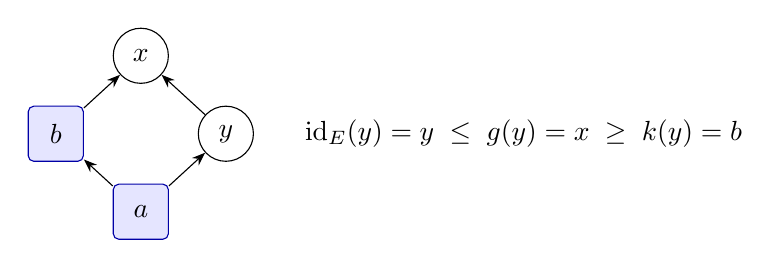
\begin{tikzpicture}[>=Stealth,scale=.9,
 old/.style={draw=blue!65!black,fill=blue!10,rounded corners=2pt,
             minimum width=7mm,minimum height=7mm},
 new/.style={draw,circle,minimum size=7mm}]
 \node[old] (a) at (0,0) {$a$};
 \node[old] (b) at (-1.2,1.1) {$b$};
 \node[new] (y) at (1.2,1.1) {$y$};
 \node[new] (x) at (0,2.2) {$x$};
 \draw[->] (a)--(b);
 \draw[->] (a)--(y);
 \draw[->] (b)--(x);
 \draw[->] (y)--(x);
 \node at (5.4,1.1)
   {$\id_E(y)=y\;\le\;g(y)=x\;\ge\;k(y)=b$};
\end{tikzpicture}
\caption{The shaded square nodes form the old sieve $A=\{a,b\}$.
Its right adjoint retraction has $r(y)=a$ and $r(x)=t=b$.
Thus $k(y)=b$ is incomparable with $y$; the common upper value $x$
supplies the two comparisons used by the relative prisms.}
\label{fig:local-diamond}
\end{figure}

\begin{theorem}[Couniversality]\label{thm:couniversal}
If $i:A\hookrightarrow E$ is a sieve of small posets with a right
adjoint retraction, then $c_n\OrdN(i)$ is a couniversal Thomason
equivalence: for every $a:\U{A}\to X$, the canonical map
\[
 X\longrightarrow X\amalg_{\U{A}}\U{E}
\]
is a Thomason equivalence.  This holds for every finite $n\ge1$ and
for $n=\infty$.
\end{theorem}

\begin{proof}
First suppose that $E$ is finite.  We use induction on
$|E\setminus A|$, simultaneously for all attaching targets $X$ and
all attaching functors $a$.  When this cardinality is zero, $j$ is an
isomorphism.  When the complement has a greatest element,
Lemma~\ref{lem:greatest-new} applies.

Otherwise the nonempty finite poset $E\setminus A$ has at least two
distinct maximal elements $x_1,x_2$: a finite poset with a unique
maximal element has that element as its greatest element.  Each $x_i$
is also maximal in $E$, since an element above a new element cannot
belong to the sieve $A$.  Put
\[
 E_1=E\setminus\{x_1\},\qquad
 E_2=E\setminus\{x_2\},\qquad
 E_{12}=E\setminus\{x_1,x_2\}.
\]
These are sieves of $E$ containing $A$; moreover
$E_1\cup E_2=E$ and $E_1\cap E_2=E_{12}$.  The restriction of $r$ to
each $E_T$, for $T=1,2,12$, still takes values in $A$ and satisfies
\eqref{eq:poset-adjunction}.  Each complement $E_T\setminus A$ is
smaller.  Define
\[
 Y_T=X\amalg_{\U{A}}\U{E_T},\qquad j_T:X\longrightarrow Y_T.
\]
By induction every $\Street j_T$ is a weak homotopy equivalence.

Corollary~\ref{cor:attachment-covers}(i), applied to the sieves
$E_1,E_2$ containing $A$ and covering $E$, identifies the canonical
maps $Y_i\to Y$ as full sieve inclusions. Their full intersection is
canonically $Y_{12}$, and they cover the objects of $Y$. These
identifications hold for the given arbitrary attaching functor $a$.

Lemma~\ref{lem:nerve-cover} now identifies the bottom pushout in the
following diagram with $\Street Y$:
\begin{equation}\label{eq:couniversal-cover-spans}
\begin{tikzcd}[column sep=large]
 \Street X \arrow[d,"\Street j_1"'] &
 \Street X \arrow[l,equal] \arrow[r,equal]
             \arrow[d,"\Street j_{12}"] &
 \Street X \arrow[d,"\Street j_2"] \\
 \Street Y_1 &
 \Street Y_{12} \arrow[l,hook] \arrow[r,hook] &
 \Street Y_2 .
\end{tikzcd}
\end{equation}
The vertical maps are the canonical maps induced by $X$, so this is
a strictly commuting map of spans.  All three are weak equivalences
by induction, and the indicated legs in both rows are
monomorphisms.  Lemma~\ref{lem:simplicial-gluing} proves that the
induced map on pushouts is a weak equivalence.  The top pushout is
$\Street X$, and its map to the bottom pushout is precisely
$\Street j$, by its restrictions to the two pieces.  This completes
the finite induction.  In particular, no compatibility between the
local cylinders on different pieces has been used.

Now let $E$ be arbitrary, and write $q=ir:E\to E$.  Since
$q^2=q$, the collection $\mathcal F$ of finite subsets $F\subset E$
with $q(F)\subset F$ is nonempty and filtered under inclusion: it
contains $\varnothing$, and finite unions remain stable.  Every
finite subset $T$ is contained in the finite stable subset
$T\cup q(T)$.  Give each $F$ its full induced order and put
$A_F=A\cap F$.  Then $A_F$ is a sieve in $F$, and stability gives
$r(F)\subset A_F$.  The restriction $r_F:F\to A_F$ is a right
adjoint retraction, since \eqref{eq:poset-adjunction} restricts to
these full subposets.  Notice that $F$ itself need not be a sieve
in $E$.

Use the restriction of $a$ to define
\[
 Y_F=X\amalg_{\U{A_F}}\U{F},\qquad j_F:X\longrightarrow Y_F.
\]
Every $j_F$ is a Thomason equivalence by the finite case.  The
inclusions $F\subset F'$ give compatible transition functors
$Y_F\to Y_{F'}$ under the same fixed $X$.  Every ordinary nerve
simplex has finite vertex support, and therefore
\[
 \OrdN E=\colim_{F\in\mathcal F}\OrdN F,
 \qquad
 \OrdN A=\colim_{F\in\mathcal F}\OrdN A_F.
\]
Applying the colimit-preserving left adjoint $c_n$ and then commuting
colimits gives
\begin{equation}\label{eq:couniversal-filtered-colimit}
 \colim_{F\in\mathcal F}Y_F
 \ \cong\ X\amalg_{\U{A}}\U{E}=Y.
\end{equation}
For clarity, the fixed copy of $X$ in this formula is essential and
legitimate: a compatible family of maps $Y_F\to Z$ consists of one
map $X\to Z$, since $\mathcal F$ is nonempty and connected, together
with compatible maps $\U{F}\to Z$ agreeing on each $\U{A_F}$.
These are exactly maps from the pushout on the right.  Under this
identification the colimit of the arrows $j_F$ is $j$.

By Lemma~\ref{lem:filtered}, $\Street$ preserves these filtered
colimits and simplicial weak homotopy equivalences are closed under
filtered colimits.  Hence $\Street j$ is a weak homotopy equivalence.
No injectivity of the transition functors $Y_F\to Y_{F'}$ is
required.  The same proof applies directly when $n=\infty$.
\end{proof}

The following unit comparison is known; see
\cite[Corollary~10.11]{AraMaltsiniotis2015},
\cite[Theorem~6.9]{Gagna2018} and
\cite[Proposition~9.2.3]{Ara2023}. We include an independent proof
using the same prism and sieve-cover method.

\begin{proposition}[The unit on every poset]\label{prop:poset-unit}
For every small poset $S$, the adjunction unit
\[
 \eta_S:\OrdN S\longrightarrow\Street\U{S}
\]
is a weak homotopy equivalence.  This assertion is natural in $S$
and holds for every finite $n\ge1$ and for $n=\infty$.
\end{proposition}

\begin{proof}
First take $S$ finite and induct on its cardinality.  If $S$ is
empty, both simplicial sets are empty and the unit is an
isomorphism.  If $S$ has a greatest element $x$, the pointwise
inequality $\id_S\le\mathrm{const}_x$ contracts $\OrdN S$.
Lemma~\ref{lem:relative-prism}, with old sieve $\varnothing$, gives
a right cylinder from $\id_{\U{S}}$ to
$c_n\OrdN(\mathrm{const}_x)$.  The latter functor factors through
$\U{\{x\}}=\Orient{0}$, the terminal strict $n$-category.
Lemma~\ref{lem:gray-nerve} therefore contracts
$\Street\U{S}$.  Both realizations are nonempty and contractible,
so $\eta_S$ is a weak homotopy equivalence.

In the remaining case choose two distinct maximal elements
$x_1,x_2$ of $S$ and put
$S_i=S\setminus\{x_i\}$ and
$S_{12}=S\setminus\{x_1,x_2\}$.  These are sieves, the two single
deletions cover $S$, and all three posets are smaller.  Their
ordinary nerves cover $\OrdN S$: a simplex belongs to a sieve
containing its last vertex.  By
Lemmas~\ref{lem:poset-pieces} and~\ref{lem:nerve-cover}, their
$\U{\,\cdot\,}$ images give a full sieve cover of $\U{S}$ and
the analogous cover of its Street nerve.  The joint zero label
identifies the intersection of the two full sieves with
$\U{S_{12}}$.  Naturality of the unit
gives a commuting map of spans
\[
\begin{tikzcd}[column sep=large]
 \OrdN S_1 \arrow[d,"\eta_{S_1}"'] &
 \OrdN S_{12} \arrow[l,hook] \arrow[r,hook]
             \arrow[d,"\eta_{S_{12}}"] &
 \OrdN S_2 \arrow[d,"\eta_{S_2}"] \\
 \Street\U{S_1} &
 \Street\U{S_{12}} \arrow[l,hook] \arrow[r,hook] &
 \Street\U{S_2} .
\end{tikzcd}
\]
The vertical maps are weak equivalences by induction; all horizontal
legs are monomorphisms.  The induced map on pushouts is a weak
equivalence by Lemma~\ref{lem:simplicial-gluing}.  Under the cover
identifications it is exactly $\eta_S$: its restriction to either
$\OrdN S_i$ agrees with that unit by naturality.  This proves the
finite case.

Finally every poset is the filtered union of its finite full
subposets.  Ordinary nerve preserves this union because each
simplex has finite support, $c_n$ preserves its colimit, and
$\Street$ preserves the resulting filtered colimit by
Lemma~\ref{lem:filtered}.  Naturality identifies $\eta_S$ with the
filtered colimit of the units on those finite subposets.
Filtered-colimit closure of simplicial weak homotopy equivalences
then proves the assertion.  This proof uses only the prism, cover,
and simplicial gluing lemmas, and in particular precedes and is
independent of the model-structure transfer.
\end{proof}

\section{Comparison for subdivided attachments}
\label{sec:attachments}

We now compare an ordinary pushout of Street nerves with the Street
nerve of an actual attachment.  All attaching functors in this section
are arbitrary.  In particular, they may identify old objects and cells.
The comparison will supply both the acyclicity of horn attachments and
the preservation of weak equivalences under boundary attachments.

We first treat a sieve $A\subset B$ whose inclusion into its upward
closure admits a right adjoint retraction.  Couniversality controls
the attachment over that upward closure; a cosieve cover then adds
the rest of $B$.  This decomposition follows the proof of
\cite[Proposition~4.3]{Thomason1980}; Theorem~\ref{thm:couniversal}
supplies its homotopy input in strict higher dimensions.  After proving
this general comparison, we identify the twice-subdivided boundaries
and horns as poset pairs with these properties.

\begin{proposition}[Attachment comparison]
\label{prop:attachment-comparison}
Let $A\subset B$ be a sieve of small posets.  Let $Z$ be its upward
closure, and suppose that $A\hookrightarrow Z$ admits a right adjoint
retraction.  For every functor $a:\U{A}\to X$ in $\nCat$, put
\[
 V_B(X)=X\amalg_{\U{A}}\U{B},\qquad
 P_B(X)=\Street X\amalg_{\Street\U{A}}\Street\U{B}.
\]
The canonical map
\begin{equation}
 \gamma_{B,X}:P_B(X)\longrightarrow\Street V_B(X)
 \label{eq:attachment-comparison}
\end{equation}
is a simplicial weak equivalence.  The map
$\Street\U{A}\to\Street\U{B}$ is a monomorphism.
The comparison is natural in every functor $f:X\to X'$ under
$\U{A}$.
\end{proposition}

\begin{proof}
First set
\[
 V_Z(X)=X\amalg_{\U{A}}\U{Z},\qquad
 P_Z(X)=\Street X\amalg_{\Street\U{A}}\Street\U{Z}.
\]
Theorem~\ref{thm:couniversal}, applied to $A\hookrightarrow Z$, says
that $X\to V_Z(X)$ belongs to $W_n$.  Applying it with old target
$\U{A}$ also says that $\U{A}\to\U{Z}$ belongs to $W_n$.
Since $A$ is a sieve in $Z$, Lemma~\ref{lem:poset-pieces} identifies
$\U{A}\to\U{Z}$ with an actual full inclusion.  Its Street nerve is
therefore a monomorphism and a weak equivalence, hence a trivial
cofibration of simplicial sets.  Its pushout
$\Street X\to P_Z(X)$ is a weak equivalence.  The canonical triangle
\[
 \begin{tikzcd}[column sep=large]
 \Street X \arrow[r] \arrow[dr] & P_Z(X) \arrow[d,"\gamma_{Z,X}"]\\
 & \Street V_Z(X)
 \end{tikzcd}
\]
then shows by two-out-of-three that $\gamma_{Z,X}$ is a weak
equivalence.

To pass from $Z$ to $B$, write
\[
 C=B\setminus A,\qquad T=Z\setminus A=Z\cap C.
\]
Both $Z$ and $C$ are cosieves in $B$, and they cover $B$: an element
outside $C$ belongs to $A\subset Z$.  Their intersection is $T$.
Lemma~\ref{lem:poset-pieces} therefore gives cosieves
$\U{Z},\U{C}\subset\U{B}$ with intersection $\U{T}$.
Apply Corollary~\ref{cor:attachment-covers}(ii) with $P=B$,
$T_1=Z$, and $T_2=C$.  Its remaining hypotheses hold because
$A\subset Z$ and $A\cap C=\varnothing$.  The canonical maps identify
\begin{equation}
 V_Z(X),\quad \U{C}\ \subset\ V_B(X),
 \qquad V_Z(X)\cap\U{C}=\U{T},
 \label{eq:attachment-fibers}
\end{equation}
as actual full cosieves and their full intersection.  These two
cosieves cover all objects of $V_B(X)$.  The corollary applies to the
given arbitrary functor $a$, including its identifications of old
objects and cells.

Apply Lemma~\ref{lem:nerve-cover} to the two cosieve covers just
obtained.  It gives ordinary simplicial pushouts
\begin{align}
 \Street\U{B}
   &=\Street\U{Z}\amalg_{\Street\U{T}}\Street\U{C},
   \label{eq:attachment-source-cover}\\
 \Street V_B(X)
   &=\Street V_Z(X)\amalg_{\Street\U{T}}\Street\U{C}.
   \label{eq:attachment-target-cover}
\end{align}
All maps from the intersections to the pieces in these covers are
monomorphisms.  Reassociating the pushout in the definition of
$P_B(X)$ using Equation~\eqref{eq:attachment-source-cover} gives
\[
 P_B(X)=P_Z(X)\amalg_{\Street\U{T}}\Street\U{C}.
\]
Under these canonical identifications, Equation~\eqref{eq:attachment-comparison}
is exactly the map induced by $\gamma_{Z,X}$ and the identity of
$\Street\U{C}$.  In particular the square
\[
 \begin{tikzcd}[column sep=large]
 P_Z(X) \arrow[r,hook] \arrow[d,"\gamma_{Z,X}"'] &
 P_B(X) \arrow[d,"\gamma_{B,X}"]\\
 \Street V_Z(X) \arrow[r,hook] & \Street V_B(X)
 \end{tikzcd}
\]
is a pushout: its lower right corner is also
$\Street V_Z(X)\amalg_{P_Z(X)}P_B(X)$.
The top horizontal map is the cobase change of the specific
monomorphism
\begin{equation}
 \Street\U{T}\hookrightarrow\Street\U{C}.
 \label{eq:comparison-monomorphism}
\end{equation}
Left properness of simplicial sets, as recorded in
Lemma~\ref{lem:simplicial-gluing}, now makes $\gamma_{B,X}$ a weak
equivalence.  Neither the map $\Street\U{A}\to\Street X$ nor the
map $\Street\U{T}\to P_Z(X)$ needs to be a monomorphism.

The remaining assertion that $\Street\U{A}\to\Street\U{B}$ is
monic follows directly from the sieve identification in
Lemma~\ref{lem:poset-pieces}.  Finally, $\gamma_{B,X}$ is defined
by the two canonical maps from $\Street X$ and $\Street\U{B}$.
For $f:X\to X'$ under $\U{A}$ these maps commute with $\Street f$
and with the induced pushout functor $V_B(X)\to V_B(X')$.
The pushout universal property therefore gives the strict naturality
square
\begin{equation}
 \begin{tikzcd}[column sep=large]
 P_B(X) \arrow[r,"\gamma_{B,X}"] \arrow[d] &
 \Street V_B(X) \arrow[d]\\
 P_B(X') \arrow[r,"\gamma_{B,X'}"'] & \Street V_B(X').
 \end{tikzcd}
 \label{eq:attachment-naturality}
\end{equation}
The comparison is thus canonical and natural, while the local
contractions used in Theorem~\ref{thm:couniversal} establish that it
is a weak equivalence.
\end{proof}

To apply the comparison to the generating maps, we now describe their
second subdivisions.  We use the classical face-chain description and
intersection retraction of \cite[Proposition~4.2]{Thomason1980}; see also
\cite[Lemmas~4.8 and~4.10]{AraMaltsiniotis2014}. The proof below records
the precise poset pair for each boundary and horn, including the empty case.

\begin{lemma}[The subdivision posets]
\label{lem:subdivision-posets}
Let $d:K\hookrightarrow\Delta[m]$ be a boundary inclusion, with $m\geq0$,
or a horn inclusion $\Lambda^k[m]\hookrightarrow\Delta[m]$, with
$m\geq1$ and $0\leq k\leq m$.  There are finite posets $A\subset B$
and a canonical identification
\[
 \Sd^2 d=\bigl(\OrdN A\hookrightarrow\OrdN B\bigr).
\]
Here $A$ is a sieve.  Its upward closure $Z$ in $B$ is a cosieve, and
$A\hookrightarrow Z$ has a right adjoint retraction.
\end{lemma}

\begin{proof}
Put $M=\{0,\ldots,m\}$ and let $P$ be the poset of its nonempty
subsets, ordered by inclusion.  The subposet $P_K$ of faces belonging
to $K$ is
\[
 P_K=
 \begin{cases}
  \{F:\varnothing\ne F\subsetneq M\},&K=\partial\Delta[m],\\[2pt]
  \{F:\varnothing\ne F\subseteq M,\ M\setminus\{k\}\nsubseteq F\},
     &K=\Lambda^k[m].
 \end{cases}
\]
Indeed, a nonempty face belongs to the horn precisely when it is
contained in $M\setminus\{j\}$ for some $j\ne k$.  Thus in the horn
case $P_K$ is obtained from $P$ by removing $M$ and
$M\setminus\{k\}$.  In both cases $P_K$ is downward closed in $P$.

The barycentric subdivision of an ordered simplicial complex has a
vertex for every nonempty face and a nondegenerate simplex for every
strict chain of such faces.  Consequently
\[
 \Sd\Delta[m]=\OrdN P,\qquad \Sd K=\OrdN P_K.
\]
One can see these identifications directly on a simplex: the vertices
of its subdivision are its nonempty subsets, and its simplices are
chains of those subsets.  The identifications agree on every face, so
they glue over the faces of $K$.  The nondegenerate simplices of
$\OrdN P$ are themselves the nonempty finite chains in $P$, with a
face obtained by deleting entries.  Applying the same description a
second time gives
\[
 \begin{split}
 B&=\{\sigma:\sigma\text{ is a nonempty chain in }P\},\\
 A&=\{\sigma\in B:\sigma\subseteq P_K\},
 \end{split}
 \qquad \sigma\leq\tau\ \Longleftrightarrow\ \sigma\subseteq\tau.
\]
This proves the claimed identifications as simplicial sets, including
degeneracies, and identifies their inclusion.

Every nonempty subchain of a chain in $A$ again belongs to $A$, so $A$
is a sieve in $B$.  Its upward closure is exactly
\[
 Z=\{\sigma\in B:\sigma\cap P_K\ne\varnothing\}.
\]
For the nontrivial implication in this equality, a face
$F\in\sigma\cap P_K$ gives $\{F\}\in A$ below $\sigma$.
Define
\[
 r:Z\longrightarrow A,\qquad r(\sigma)=\sigma\cap P_K.
\]
This is a nonempty chain, is monotone under inclusion, and fixes $A$.
For $\alpha\in A$ and $\sigma\in Z$ one has
\[
 \alpha\subseteq\sigma
 \quad\Longleftrightarrow\quad
 \alpha\subseteq\sigma\cap P_K=r(\sigma).
\]
This is precisely the right adjunction to $A\hookrightarrow Z$.

When $m=0$ and $K=\partial\Delta[0]$, the poset $B$ is a singleton
and $A=Z=\varnothing$; the asserted adjunction is the identity of the
empty poset.  For a one-dimensional horn, $P_K=\{\{k\}\}$, so $A$
is a singleton and $Z$ consists of the chains containing the face
$\{k\}$.  These cases are included in the formulas above.  There are
no zero-dimensional horn generators.
\end{proof}

\begin{remark}
For the zero-dimensional boundary, $A=Z=T=\varnothing$ and $B=C$
is a singleton.  Thus $V_Z(X)=X$ and $\gamma_{Z,X}=\id$; the two
cosieves of $V_B(X)=X\amalg\U{B}$ are disjoint.  The comparison in
Proposition~\ref{prop:attachment-comparison} is then the isomorphism
\[
 \Street X\amalg\Delta[0]\ \cong\ \Street(X\amalg\U{B}).
\]
\end{remark}

\begin{corollary}[Horn attachments are acyclic]
\label{cor:horn-acyclic}
For every horn inclusion $d\in J$, every pushout of $L_n d$ belongs
to $W_n$.
\end{corollary}

\begin{proof}
Use the pair $A\subset B$ from Lemma~\ref{lem:subdivision-posets},
so that $L_n d$ is $\U{A}\to\U{B}$.
The inclusion $\OrdN A\to\OrdN B$ is a weak equivalence: the horn
inclusion is a simplicial weak equivalence, and subdivision preserves
weak equivalences.  The latter follows by naturality and
two-out-of-three from the objectwise weak equivalence
$\Sd\to\id$ of \cite[Theorem~4.5]{AraMaltsiniotis2014}.
Naturality of the adjunction unit gives a square
\[
 \begin{tikzcd}[column sep=large]
 \OrdN A \arrow[r] \arrow[d] & \OrdN B \arrow[d]\\
 \Street\U{A} \arrow[r] & \Street\U{B}.
 \end{tikzcd}
\]
The vertical maps are weak equivalences by
Proposition~\ref{prop:poset-unit}.  Two-out-of-three makes the lower
map a weak equivalence, and it is monic by
Proposition~\ref{prop:attachment-comparison}.  Thus it is a
simplicial trivial cofibration.  For any attaching functor
$\U{A}\to X$, its pushout $\Street X\to P_B(X)$ is a weak
equivalence.  The composite
\[
 \Street X\longrightarrow P_B(X)
   \xrightarrow{\gamma_{B,X}}\Street V_B(X)
\]
is the nerve of the attachment $X\to V_B(X)$, and both factors are
weak equivalences.  This is exactly the assertion that the
attachment belongs to $W_n$.
\end{proof}

\begin{corollary}[Invariance under attachment]
\label{cor:attachment-invariance}
Let $d\in I\cup J$, write $L_n d$ as $\U{A}\to\U{B}$ using
Lemma~\ref{lem:subdivision-posets}, and let $f:X\to X'$ belong to
$W_n$.  For every $a:\U{A}\to X$, the induced functor
\[
 X\amalg_{\U{A}}\U{B}
 \longrightarrow X'\amalg_{\U{A}}\U{B},
\]
where the second attaching functor is $fa$, belongs to $W_n$.
\end{corollary}

\begin{proof}
The map $\Street X\to P_B(X)$ is a monomorphism, being the
cobase change of $\Street\U{A}\hookrightarrow\Street\U{B}$.
There is a canonical pushout identification
\[
 P_B(X')=\Street X'\amalg_{\Street X}P_B(X).
\]
Left properness of simplicial sets therefore makes
$P_B(X)\to P_B(X')$ a weak equivalence, since $\Street f$ is one.
In the naturality square of Equation~\eqref{eq:attachment-naturality}, both horizontal
maps are weak equivalences by
Proposition~\ref{prop:attachment-comparison}.  Two-out-of-three
implies that its right vertical map is a weak equivalence.  This is
the nerve of the asserted functor.
\end{proof}

\section{The model structure and the Quillen equivalence}
\label{sec:transfer}

Fix $n\in\{1,2,\ldots,\infty\}$.
Corollary~\ref{cor:horn-acyclic} supplies the acyclic horn attachments
needed for the model axioms; Corollary~\ref{cor:attachment-invariance}
supplies the invariance under boundary attachment needed for left
properness. We extend these statements through transfinite compositions,
then prove the Quillen equivalence by checking the unit on arbitrary
simplicial sets. Write
\[
 L_n=c_n\Sd^2,\qquad R_n=\Ex^2\Street,
 \qquad L_n\dashv R_n.
\]
We use the Kan--Quillen model structure on $\sSet$, with weak
equivalences $W_{\mathrm{KQ}}$, fibrations
$\mathrm{Fib}_{\mathrm{KQ}}$, and generating sets
\begin{align*}
 I&=\{\partial\Delta[m]\hookrightarrow\Delta[m]\mid m\geq0\},\\
 J&=\{\Lambda^k[m]\hookrightarrow\Delta[m]\mid m\geq1,
                    \ 0\leq k\leq m\}.
\end{align*}
In particular, $\partial\Delta[0]=\varnothing$.

We first record the classical simplicial facts needed to identify the
weak equivalences.  The last-vertex transformation
$\ell:\Sd\longrightarrow\id$ is an objectwise weak equivalence
\cite[Theorem~4.5]{AraMaltsiniotis2014}.  Its mate
$j:\id\longrightarrow\Ex$ is also an objectwise weak equivalence
\cite[Theorem~III.4.6]{GoerssJardine1999}.  The latter assertion is
a theorem about subdivision and extension, and is not a formal
consequence of being a mate.  Both statements apply to every
simplicial set independently of the model structure being constructed.
For a map $f:K\to K'$, naturality gives
\[
 j_{K'}f=(\Ex f)j_K.
\]
Two-out-of-three therefore proves that $\Ex$ preserves and reflects
weak equivalences.  Similarly, naturality of $\ell$ shows that $\Sd$
preserves and reflects weak equivalences.  In particular,
\begin{equation}\label{eq:model-classes}
 \begin{split}
 W_n&=\Street^{-1}(W_{\mathrm{KQ}})
        =R_n^{-1}(W_{\mathrm{KQ}}),\\
 F_n&=R_n^{-1}(\mathrm{Fib}_{\mathrm{KQ}}),\qquad
 C_n={}^{\perp}(F_n\cap W_n).
 \end{split}
\end{equation}
Here ${}^{\perp}$ denotes the left lifting property.  The class $W_n$
has two-out-of-three and is closed under retracts.  By
Lemma~\ref{lem:filtered}, it is also closed under filtered colimits of
arrows, without any injectivity requirement on their transition maps.

For a set $\mathcal S$ of maps, write $\mathcal S\text{-inj}$ for the
maps with the right lifting property against $\mathcal S$, and
$\mathcal S\text{-cof}={}^{\perp}(\mathcal S\text{-inj})$.
A relative $\mathcal S$-cell map is a transfinite composite of
pushouts of coproducts of members of $\mathcal S$.

\begin{lemma}[Transfinite horn attachments]\label{lem:transfinite-horns}
Every relative $L_nJ$-cell map belongs to $W_n$.
\end{lemma}

\begin{proof}
Corollary~\ref{cor:horn-acyclic} proves the assertion for one
attachment, with an arbitrary attaching target.  A set of simultaneous
attachments may be well ordered and attached one at a time: at each
stage use the given map from its source into the original target,
followed by the map to the current stage.  The universal property of
the resulting colimit is the universal property of the pushout of
the coproduct.  Thus it suffices to consider a continuous ordinal
sequence $(X_\alpha)_{\alpha\leq\lambda}$ in which each successor
map is a single such attachment.

By transfinite induction, $X_0\to X_\alpha$ belongs to $W_n$ for
every $\alpha$.  The assertion at zero is the identity, and the
successor step is composition with the weak equivalence supplied by
Corollary~\ref{cor:horn-acyclic}.  If $\beta$ is a nonzero limit
ordinal, the ordinal of stages $\alpha<\beta$ is filtered.  Apply
Lemma~\ref{lem:filtered} to the diagram of arrows
$X_0\to X_\alpha$.  Its colimit is
$X_0\to\colim_{\alpha<\beta}X_\alpha=X_\beta$, because the
colimit of the constant source diagram is $X_0$.  This proves the
limit step and the lemma.
\end{proof}

\begin{proposition}[The transferred model structure]\label{prop:model-structure}
The classes $(C_n,W_n,F_n)$ in
\eqref{eq:model-classes} form a combinatorial model structure on
$\nCat$, cofibrantly generated by $(L_nI,L_nJ)$.
\end{proposition}

\begin{proof}
The underlying category is locally presentable, and hence complete
and cocomplete, by Lemma~\ref{lem:filtered}.  We describe the small
object argument to make clear that the factorizations have no
restriction on their sources.  For either set
$\mathcal S=L_nI$ or $\mathcal S=L_nJ$, choose an infinite regular
cardinal $\kappa$ such that every domain in $\mathcal S$ is
$\kappa$-presentable.  Such a common bound exists because the
category is locally presentable and $\mathcal S$ is a set.

Given any map $X\to Y$, start with $X_0=X$.  At stage $\alpha+1$
attach to $X_\alpha$ one copy of the codomain of each member of
$\mathcal S$ for every commutative square from that member to
$X_\alpha\to Y$.  This is a set of squares, by local smallness.
Use colimits at limit stages.  The resulting factorization is
\[
 X\xrightarrow{i}X_\kappa\xrightarrow{p}Y.
\]
Here $i$ is a relative $\mathcal S$-cell map and
$p\in\mathcal S\text{-inj}$.  Indeed a map from a generating
domain to $X_\kappa$ factors through some $X_\alpha$, since the
ordinal $\kappa$ is $\kappa$-filtered.  Its lifting square against
$p$ was therefore attached at stage $\alpha+1$, which supplies the
required lift.  The construction may be made functorial by using
all squares at each stage.

Pushouts, transfinite composites, and retracts of maps with a fixed
left lifting property retain that property.  Consequently every
relative $\mathcal S$-cell map lies in $\mathcal S\text{-cof}$.
Conversely, if $u:A\to B$ belongs to $\mathcal S\text{-cof}$,
factor it as $A\xrightarrow{i}Z\xrightarrow{p}B$ by the construction
above.  The square with top map $i$, left map $u$, right map $p$,
and bottom map $\id_B$ admits a diagonal $s:B\to Z$.  The equations
$su=i$ and $ps=\id_B$ exhibit $u$ as a retract of $i$ in the arrow
category, with the source fixed at $A$.  Thus the construction gives
the weak factorization system
\[
 (\mathcal S\text{-cof},\mathcal S\text{-inj}),
\]
and its left class consists exactly of retracts of relative
$\mathcal S$-cell maps.

The adjunction identifies lifting squares and their fillers.  The
Kan--Quillen lifting characterizations therefore give exactly
\begin{align}
 (L_nI)\text{-inj}
   &=R_n^{-1}(I\text{-inj})=F_n\cap W_n,
       \label{eq:boundary-injectives}\\
 (L_nJ)\text{-inj}
   &=R_n^{-1}(J\text{-inj})=F_n.
       \label{eq:horn-injectives}
\end{align}
In the first equality of classes on the right of
\eqref{eq:boundary-injectives}, we used the equality of the two
definitions of $W_n$ proved above.  The first weak factorization
system is consequently $(C_n,F_n\cap W_n)$.

Let $\mathcal D=(L_nJ)\text{-cof}$.  As $F_n\cap W_n\subseteq F_n$,
one has $\mathcal D\subseteq C_n$.  Lemma~\ref{lem:transfinite-horns} and
retract closure give $\mathcal D\subseteq W_n$ as well.  To prove the
reverse inclusion, take $u:A\to B$ in $C_n\cap W_n$ and factor it
by the second small object argument as
$A\xrightarrow{i}Z\xrightarrow{p}B$, with $i\in\mathcal D$ and
$p\in F_n$.  Since $i$ and $u=pi$ belong to $W_n$,
two-out-of-three gives $p\in F_n\cap W_n$.  The lifting property
of $u\in C_n$ now supplies $s:B\to Z$ with $su=i$ and
$ps=\id_B$.  The same fixed-source retract diagram puts $u$ in
$\mathcal D$.  We have proved
\[
 \mathcal D=C_n\cap W_n.
\]
Thus the second weak factorization system is $(C_n\cap W_n,F_n)$.
Together with two-out-of-three and retract closure for $W_n$, these
are all the model axioms.  Local presentability and the displayed
generating sets make the model structure combinatorial.
\end{proof}

\begin{proposition}[Properness]\label{prop:properness}
The model structure of Proposition~\ref{prop:model-structure} is
left and right proper.
\end{proposition}

\begin{proof}
For right properness, let $p:Y\to Z$ belong to $F_n$ and let
$w:Z'\to Z$ belong to $W_n$.  The right adjoint $R_n$ carries the
pullback $Y\times_Z Z'$ to the corresponding simplicial pullback.
Its map to $R_nY$ is a weak equivalence by right properness of the
Kan--Quillen model structure, since $R_np$ is a Kan fibration and
$R_nw$ is a weak equivalence.  The definition of $W_n$ then gives
$Y\times_Z Z'\to Y$ in $W_n$.

For left properness, first let $i:X\to Y$ be a relative
$L_nI$-cell map and let $w:X\to X'$ belong to $W_n$.  As in
Lemma~\ref{lem:transfinite-horns}, write $i$ as a continuous
sequence of individual boundary attachments $X_\alpha$ starting
at $X$.  Put $X'_\alpha=X'\amalg_X X_\alpha$.
We prove by induction that $X_\alpha\to X'_\alpha$ belongs to
$W_n$.  This is $w$ at stage zero.  At a successor stage, the
second attachment has the first attaching map followed by
$X_\alpha\to X'_\alpha$, so
Corollary~\ref{cor:attachment-invariance} proves the induction
step.  At a nonzero limit ordinal, both sequences are their
colimits, and Lemma~\ref{lem:filtered} gives the assertion.  Hence
$Y\to X'\amalg_XY$ belongs to $W_n$.

For a general $i:X\to Y$ in $C_n$, the first small object
factorization and its lifting retract, used in
Proposition~\ref{prop:model-structure}, express $i$ as a retract
of a relative $L_nI$-cell map $j:X\to Z$ with the same source.
Explicitly there are $s:Y\to Z$ and $p:Z\to Y$ with
$si=j$, $pj=i$, and $ps=\id_Y$.  Cobase change along $w$ gives
the corresponding maps $s'$ and $p'$ between
$X'\amalg_XY$ and $X'\amalg_XZ$, with $p's'=\id$.
Thus the arrow $Y\to X'\amalg_XY$ is a retract of
$Z\to X'\amalg_XZ$.  The latter is in $W_n$ by the preceding
paragraph, and so is the former.  Both properness arguments apply
to arbitrary objects; no cofibrancy or fibrancy condition on the
base objects was used.
\end{proof}

Let $\eta_T:T\to\Street c_nT$ denote the unit of
$c_n\dashv\Street$.  The poset unit of
Proposition~\ref{prop:poset-unit} is the case $T=\OrdN E$.
The next proposition extends the required comparison to all
simplicial sets after two subdivisions.

\begin{proposition}[The unit after two subdivisions]\label{prop:subdivided-unit}
For every simplicial set $K$, the canonical map
\begin{equation}\label{eq:subdivided-unit}
 \theta_K=\eta_{\Sd^2K}:\Sd^2K\longrightarrow\Street L_nK
\end{equation}
is a weak equivalence.
\end{proposition}

\begin{proof}
For $K=\Delta[m]$ and $K=\partial\Delta[m]$,
Lemma~\ref{lem:subdivision-posets} identifies $\Sd^2K$ with the
ordinary nerve of a poset.  The assertion is therefore
Proposition~\ref{prop:poset-unit}.  It also holds for the empty
simplicial set: $c_n\varnothing$ is the empty strict category,
whose Street nerve is empty.

Every simplicial set is obtained from the empty set by a
continuous transfinite sequence of boundary attachments.  One
construction orders its nondegenerate simplices by dimension and
well orders those in each dimension.  The boundary of a simplex
then maps into the stage already constructed.  That attaching
map may identify vertices or faces, or send faces to degenerate
simplices.  The construction still recovers $K$, by the unique
expression of each simplex as a degeneracy of a nondegenerate
simplex.

Consider one successor step
\[
 K_+=K_0\amalg_{\partial\Delta[m]}\Delta[m]
\]
and assume the assertion for $K_0$.  Write
\[
 V=\Sd^2K_0,\qquad A=\Sd^2\partial\Delta[m],
 \qquad B=\Sd^2\Delta[m].
\]
Here $A,B,V$ are simplicial sets; the representing posets for $A,B$
will be denoted by $E,F$ below. Since subdivision is a left adjoint,
$\Sd^2K_+=V\amalg_A B$.  Naturality of $\eta$ gives a map of
spans and hence the map
\begin{equation}\label{eq:unit-gluing-map}
 q:V\amalg_A B\longrightarrow
       \Street c_nV\amalg_{\Street c_nA}\Street c_nB.
\end{equation}
The three maps on the objects of these spans are weak
equivalences: on $V$ by induction and on $A,B$ by the simplex and
boundary cases.  The leg $A\to B$ is a simplicial monomorphism.
Writing $A=\OrdN E$ and $B=\OrdN F$ as in
Lemma~\ref{lem:subdivision-posets}, the inclusion $E\subseteq F$
is a sieve; Lemma~\ref{lem:poset-pieces} makes
$c_nA\to c_nB$ a sieve inclusion.  Consequently
$\Street c_nA\to\Street c_nB$ is also a monomorphism.
Lemma~\ref{lem:simplicial-gluing}, applied with these two
specified monomorphic legs, proves that $q$ is a weak equivalence.
It requires no monomorphism condition on $A\to V$.

Apply Proposition~\ref{prop:attachment-comparison} to the
arbitrary attaching functor $c_nA\to c_nV$.  It says that
\begin{equation}\label{eq:unit-attachment-comparison}
 t:\Street c_nV\amalg_{\Street c_nA}\Street c_nB
       \longrightarrow
       \Street(c_nV\amalg_{c_nA}c_nB)
\end{equation}
is a weak equivalence.  Because $c_n$ preserves colimits, the
target is $\Street c_n(V\amalg_A B)$.
The composite $tq$ is exactly $\eta_{V\amalg_A B}$: on each of
the two pushout legs $V$ and $B$ this follows from naturality of
$\eta$, and equality on those legs determines the map from the
pushout.  Thus the actual canonical map
$\theta_{K_+}$ is a weak equivalence.  This also explains why
noninjective boundary maps cause no change to the argument.

At a nonzero limit ordinal, $\Sd^2$ and $L_n$ preserve the
colimit as left adjoints, while $\Street$ preserves the filtered
colimit by Lemma~\ref{lem:filtered}.  Therefore the unit at that
stage is the filtered colimit of the previous units; it is a weak
equivalence by the same lemma.  Transfinite induction proves
\eqref{eq:subdivided-unit} for every $K$.  The poset descriptions
used in this proof concern the simplex and boundary pieces only.
\end{proof}

\begin{theorem}[Quillen equivalence]\label{thm:quillen-equivalence}
The adjunction
\[
 L_n:\sSet_{\mathrm{KQ}}\rightleftarrows
       (\nCat,C_n,W_n,F_n):R_n
\]
is a Quillen equivalence.
\end{theorem}

\begin{proof}
Equations~\eqref{eq:boundary-injectives} and
\eqref{eq:horn-injectives} show that $R_n$ preserves fibrations
and trivial fibrations, so this is a Quillen adjunction.

Set $S=\Sd$ and $T=\Ex$, and let $a_K:K\to TSK$ be the unit of
$S\dashv T$. The mate identity is
\[
 j_K=T(\ell_K)a_K:K\longrightarrow TK.
\]
The independently cited theorem above makes $j_K$ a weak equivalence.
Since $\ell_K$ is a weak equivalence and $T$ preserves weak
equivalences, $T(\ell_K):TSK\to TK$ is also one. Hence $a_K$ is a
weak equivalence for every simplicial set $K$, by two-out-of-three.
In particular, $a_{SK}:SK\to TS^2K$ is a weak equivalence. The unit
of $S^2\dashv T^2$ is
\[
 b_K=T(a_{SK})a_K:K\longrightarrow T^2S^2K,
 \qquad T(a_{SK}):TSK\longrightarrow T^2S^2K.
\]
Thus $b_K$ is a weak equivalence because $T$ preserves weak equivalences.
Composition is written with the rightmost map applied first.

The unit of the composite adjunction $L_n\dashv R_n$ is
\[
 u_K=T^2(\theta_K)b_K:
       K\longrightarrow T^2\Street c_nS^2K=R_nL_nK.
\]
Proposition~\ref{prop:subdivided-unit}, preservation of weak
equivalences by $T$, and the preceding calculation show that
$u_K$ is a weak equivalence for every $K$.
For any strict functor $f:L_nK\to Y$, its simplicial adjunct is
\[
 f^\sharp=R_n(f)u_K:K\longrightarrow R_nY.
\]
Using the definition of $W_n$ and two-out-of-three now gives
\[
 f\in W_n
 \quad\Longleftrightarrow\quad
 R_n(f)\in W_{\mathrm{KQ}}
 \quad\Longleftrightarrow\quad
 f^\sharp\in W_{\mathrm{KQ}}.
\]
This equivalence holds for every $K$ and $Y$.  In particular it
holds for cofibrant $K$ and fibrant $Y$, which is the
Quillen-equivalence criterion.  Together with
Propositions~\ref{prop:model-structure} and~\ref{prop:properness},
this proves all the asserted model-categorical conclusions for
each finite $n\geq1$ and for $n=\infty$.
\end{proof}

\appendix
\section{Presentations and local finite presentability}
\label{app:presentability}

We give a direct proof of the presentability assertion used in
Lemma~\ref{lem:filtered}. The point requiring care is that an equation
between boundary cells can create new composable pairs. Presentations
must therefore generate defined terms and equations together; taking
an ordinary quotient of the cells already present would not suffice.
All sets and constructions below lie in the fixed universe.

\subsection{Operations and their domains}

Fix $n\in\{1,2,\ldots,\infty\}$, with $\infty$ denoting $\omega$.
Use one sort $C_d$ for each $0\le d\le n$, or for each nonnegative
integer $d$ when $n=\infty$. The total operations are
\[
 s_d,t_d:C_d\longrightarrow C_{d-1}\quad(d>0),
 \qquad
 e_d:C_d\longrightarrow C_{d+1}\quad(d<n).
\]
For $0\le k<d$, write $s_k^d,t_k^d$ for the iterated source and
target, and $e_k^d$ for the iterated identity from sort $k$ to
sort $d$. Each is a finite term. There is a binary partial operation
$*_k^d$ on $C_d$ whose domain is exactly
\begin{equation}\label{eq:pres-domain}
 s_k^d(x)=t_k^d(y).
\end{equation}
Thus $x*_k^d y$ means $x$ after $y$. Superscripts will be omitted
when the sort is clear.

For clarity, the equations imposed are the usual strict globular
category equations. Globularity and the identity boundary equations are
\[
 s_{d-1}s_d=s_{d-1}t_d,\qquad
 t_{d-1}s_d=t_{d-1}t_d,\qquad
 s_{d+1}e_d=\id=t_{d+1}e_d.
\]
The globularity equations apply for $2\le d\le n$, and the identity
boundary equations for $0\le d<n$; when $n=\infty$, there is no upper
bound on these integer indices.
For a pair satisfying \eqref{eq:pres-domain}, the composition boundary
equations are
\[
\begin{array}{ll}
 s_d(x*_{d-1}y)=s_d(y),&
 t_d(x*_{d-1}y)=t_d(x),\\[2pt]
 s_d(x*_k y)=s_d(x)*_k s_d(y),&
 t_d(x*_k y)=t_d(x)*_k t_d(y)\quad(k<d-1).
\end{array}
\]
For each $k$, associativity is imposed on triples with
$s_k(x)=t_k(y)$ and $s_k(y)=t_k(z)$. The unit equations are
\[
 x*_k e_k^d(s_k^d x)=x,\qquad
 e_k^d(t_k^d x)*_k x=x.
\]
Identities preserve every lower composition:
$e_d(x*_k^d y)=e_d(x)*_k^{d+1}e_d(y)$ whenever the pair is
composable and $d<n$.

Interchange, for $k<l<d$, is
\begin{equation}\label{eq:pres-interchange}
 (x*_l y)*_k(z*_l w)=(x*_k z)*_l(y*_k w).
\end{equation}
Its guard includes all four inner matching equations:
\begin{equation}\label{eq:pres-interchange-guard}
\begin{aligned}
 s_l^d(x)&=t_l^d(y),&\qquad s_l^d(z)&=t_l^d(w),\\
 s_k^d(x)&=t_k^d(z),& s_k^d(y)&=t_k^d(w).
\end{aligned}
\end{equation}
These equations also imply the two outer matching conditions.
For the left side, globularity gives
\[
 s_k^d(x*_l y)=s_k^d(x)=s_k^d(y),\qquad
 t_k^d(z*_l w)=t_k^d(z)=t_k^d(w).
\]
For the right side, the iterated boundary formulas give
\[
\begin{split}
 s_l^d(x*_k z)&=s_l^d(x)*_k^l s_l^d(z),\\
 t_l^d(y*_k w)&=t_l^d(y)*_k^l t_l^d(w).
\end{split}
\]
The lower-dimensional composites in these formulas are defined by
the last two equations of \eqref{eq:pres-interchange-guard} and
globularity. The first two equations then make their values equal.
Thus the guard describes an ordinary composable array, not an
additional restriction on interchange.
Definedness of the right-hand side alone is not used to infer
the guard or definedness of the left-hand side.

These are a set of conditional equations with finite terms and
finitely many premises. In the $\omega$ case the sorts and operation
symbols are countable, but no operation or equation involves infinitely
many arguments. The resulting models are precisely strict globular
$n$-categories. For finite $n$, adjoining iterated identities above
dimension $n$ gives the convention used in the body of the paper.

\subsection{Defined terms and presentations}

A \emph{sorted set of generators} $G$ assigns a dimension to each
generator. Let $T(G)$ be the set of all finite well-sorted raw terms
in these generators and the operation symbols. A formal composite
belongs to $T(G)$ even if its boundary equation is not yet known;
it will represent a cell only after being declared defined.

Let $R$ be a set of equations between raw terms of the same sort.
An equation in $R$ is a \emph{strong equation}: its interpretation
requires both terms to be defined and their values to agree. In
particular, $t=t$ can be used to require that a particular term be
defined.

\begin{lemma}[Strict-category presentations]
\label{lem:strict-presentations}
For every sorted set $G$ and every set $R$ of strong equations,
there is a small strict $n$-category $P(G,R)$ such that, naturally in
$Y$, strict functors $P(G,R)\to Y$ correspond to sorted assignments
of the generators to cells of $Y$ satisfying $R$.
\end{lemma}

\begin{proof}
Generate simultaneously judgments $\mathsf D(t)$ and $t=u$,
meaning that $t$ is defined and that $t,u$ are defined with the
same value. Use the following rules.
\begin{enumerate}[label=(\roman*)]
\item Every generator is defined, and each member of $R$ is an
equation.
\item An equation $t=u$ implies $\mathsf D(t)$ and $\mathsf D(u)$.
Definedness of an operation term implies definedness of all its
arguments. Definedness of $x*_k y$ also implies its matching
equation \eqref{eq:pres-domain}.
\item Total operations applied to defined arguments give defined
terms. Defined arguments satisfying \eqref{eq:pres-domain} give a
defined composite.
\item Equality is symmetric and transitive. Reflexivity is the
rule $\mathsf D(t)\Rightarrow t=t$; it is not imposed on undefined
raw terms.
\item Equal arguments transport definedness and equality through
an operation. Precisely, from $t_i=u_i$ for all arguments and
$\mathsf D(f(t_1,\ldots,t_r))$, infer
$\mathsf D(f(u_1,\ldots,u_r))$ and equality of these two operation
terms.
\item Impose every ground instance of the strict category equations
above when its arguments are defined and its stated matching
conditions hold. The conclusion is equality of the two sides and
therefore definedness of both. In particular, interchange retains
all four conditions in \eqref{eq:pres-interchange-guard}.
\end{enumerate}
Globularity, identity boundary and unit equations require just
definedness of their variables. Composition boundary equations and
preservation of composition by identities require
\eqref{eq:pres-domain}; associativity requires its two matching
equations. Thus every rule has finitely many premises. All rules
are sound in a strict category, including the definedness conclusions
in the last rule.

Start with the assumptions and repeatedly add the conclusions of
all applicable rules. The union of the finite stages is the least
closed set of judgments: any rule's finitely many premises occur
together at some stage. In particular, every resulting judgment
has a finite derivation. This construction involves a set of
judgments, since the signature and the set of raw finite terms
are sets.

Let $P(G,R)_d$ be the defined terms of sort $d$ modulo derivable
equality. The equality rules give an equivalence relation on this
set. Total operations descend by rules (iii) and (v). For the
partial operations, suppose the boundary classes of $[x]$ and
$[y]$ match. Total boundary terms are defined, so equality of
their classes means that $s_k(x)=t_k(y)$ is derivable. Rule (iii)
then declares $x*_k y$ defined.

This construction does not depend on the representatives. Indeed,
if $x=x'$ and $y=y'$ are derivable, total-operation congruence gives
\[
 s_k(x)=s_k(x'),\qquad t_k(y)=t_k(y').
\]
The matching equality for $x,y$ therefore gives the matching
equality for $x',y'$. Rule (iii) defines both composites, and
rule (v) equates them. Conversely, rule (ii) ensures that every
admitted composite has matching boundaries. The operation domain
in the quotient is consequently exactly the set of matching
pairs. Rule (vi) gives all the strict category laws there.

Now let an assignment $G\to Y$ satisfy $R$. Induction on derivations
shows that each term declared defined evaluates in $Y$ and each
derived equation has equal values. For rule (v), equal arguments
have identical boundary values, so existence of one partial
operation value entails existence of the other. Evaluation
therefore descends to a strict functor $P(G,R)\to Y$.
It is unique by induction on terms, since definedness is hereditary
to subterms and the images of the generators are fixed. Conversely,
every strict functor gives such an assignment. This proves the
universal property.

The constructed object is small. There is no inconsistency
obstruction: the strict category with one cell in each sort
satisfies every strong equation under the unique assignment.
If $G$ is empty then there are no raw ground terms, since all
operations have positive arity. The construction gives the empty
strict category in that case.
\end{proof}

\begin{remark}\label{rem:presentations-create-composites}
The simultaneous construction is necessary even for ordinary
categories. If the source and target of the free arrow are
identified, its presentation must create the square of the arrow
and all higher powers. These are not obtained by merely identifying
members of the original set of cells. Rule (iii) creates them as
soon as their boundary equalities become derivable.
\end{remark}

\subsection{Limits, colimits, and finite presentations}

\begin{proposition}[Local finite presentability]
\label{prop:strict-presentability}
For every $1\le n\le\infty$, the category $\nCat$ is locally small,
complete, cocomplete, and locally finitely presentable. Filtered
colimits are computed on cells. Every set of objects has a common
infinite regular presentability bound.
\end{proposition}

\begin{proof}
\emph{Colimits.}
For a small diagram $X:I\to\nCat$, use a generator $[i,a]$ for
each cell $a$ of each $X_i$. Impose all its operation-table
equations:
\[
\begin{split}
 s([i,a])&=[i,s(a)],\qquad t([i,a])=[i,t(a)],\\
 e([i,a])&=[i,e(a)],\qquad
 [i,a]*_k[i,b]=[i,a*_k b]
\end{split}
\]
where the last equation is included for every defined composite.
For each arrow $f:i\to j$ also impose
$[i,a]=[j,X(f)(a)]$. All these generators and equations form
sets. By Lemma~\ref{lem:strict-presentations}, maps from this
presentation to $Y$ are exactly compatible families of strict
functors $X_i\to Y$. It is therefore the colimit.

\emph{Limits and local smallness.}
In each dimension, take the set of compatible families in the
diagram. Source, target and identity are coordinatewise.
Two families have matching boundaries exactly when their
coordinates do, so coordinatewise composition is defined on
exactly the required domain and again gives a compatible family.
All laws and the limit universal property hold coordinatewise.
This includes the empty limit, with a singleton in each sort.
Strict functors form a subset of the product of the sets of
cell maps, so the category is locally small.

\emph{Filtered colimits and finite witnesses.}
For a filtered diagram, form the colimit of each set of cells.
Finitely many representatives occur at a common stage. If a
matching equation holds in the colimit, it holds at a later
common stage, where the composite can be formed. A further
common stage proves independence of choices. Each category law
holds at a stage containing its finite tuple and its matching
equations. This constructs the colimit with its universal
property, without any injectivity assumption on transition maps.

We will also use the finite-term version of this argument.
If finitely many assigned generator values make a finite
collection of terms defined and satisfy specified equations in
the colimit, these facts hold at a common stage. Induct on the
finitely many subterms: first lift the arguments, then the
boundary equality needed for a partial composite, and then
the composite. Finally lift the required equalities. Each step
uses the equality criterion for filtered colimits of sets.

\emph{Finite presentations.}
If $G$ and $R$ are finite, a map
$P(G,R)\to\colim_iX_i$ is an assignment of finitely many generator
values satisfying finitely many strong equations. The preceding
finite-term argument lifts that assignment and all the relations
to a single stage. Lemma~\ref{lem:strict-presentations} then
gives a functor to that stage. If two stage functors become
equal in the colimit, their values on the finite set $G$ agree
at a later common stage; their entire functors agree there by
the presentation universal property. Thus
\[
 \colim_i\Hom(P(G,R),X_i)
       \ \cong\ \Hom(P(G,R),\colim_iX_i).
\]
Hence every finite presentation is finitely presentable.
This does not assert that it has finitely many cells.

\emph{A generating set of finite presentations.}
Every strict category $X$ has its full cell presentation:
one generator $g_a$ for each cell and all operation-table
equations. Evaluation identifies its presented category with
$X$. Indeed it is onto, and induction on a defined term,
using the operation-table equations, equates that term to
the generator of its value. This also proves injectivity.

Write this presentation as $(G_X,R_X)$. Consider all finite
pairs $(G_0,R_0)$ with $G_0\subseteq G_X$, $R_0\subseteq R_X$,
and with every generator occurring in $R_0$ contained in
$G_0$. Ordered by inclusion, these pairs form a nonempty
filtered poset: the empty pair is allowed, and finite unions
give upper bounds. Their presented categories have colimit
$P(G_X,R_X)$. To verify this, a compatible family of maps
from the finite presentations assigns a value to every
generator and enforces every relation, since each appears
in some finite pair. The presentation universal property
gives exactly a map from $P(G_X,R_X)$.

The finite pairs need not be closed under all operations.
Finite presentations themselves supply the required closures.
There is a set of finite presentation types: use finite
numbered generator sets with specified sorts and finite sets
of raw term equations. Thus every object is a filtered
colimit of objects from a set of finitely presentable objects.
Together with cocompleteness, this is local finite
presentability. The same reasoning applies to the countable
signature in the $\omega$ case.

\emph{A common regular bound.}
More generally, if $G$ and $R$ have cardinality less than an
infinite regular cardinal $\kappa$, the same proof makes
$P(G,R)$ $\kappa$-presentable. In a $\kappa$-filtered diagram
one lifts fewer than $\kappa$ generator values and the
finitely many subterms of each of fewer than $\kappa$
relations. All stage, morphism and equality witnesses involved
form a diagram of size less than $\kappa$, so a cocone places
them at one stage. Equality of maps is detected by the
fewer than $\kappa$ generator equalities in the same way.

The full cell presentation of $X$ has cardinality at most
\[
 \max\left\{\aleph_0,\left|\coprod_d X_d\right|\right\},
\]
because the signature is countable and operations have arity
at most two. Choose a larger infinite regular cardinal.
The preceding argument makes $X$ presentable at that bound.
For a set of objects, bound the cardinalities of all their
full presentations first and choose one larger infinite
regular cardinal. This gives the claimed common bound.
\end{proof}

\section{Relation to the weak-groupoid expansion method}
\label{sec:context}

The elementary-expansion theorem of \cite{OpenAI2026} concerns
models of a fixed Grothendieck coherator in the Ara--Henry convention.
Its Theorem~1.1 asserts that, for a cellular model \(X\), freely adjoining
a parallel \(m\)-cell and an \((m+1)\)-cell joining it to a prescribed
cell preserves components and based homotopy groups.  Cellular inputs
include transfinite cellular presentations; its Corollary~5.1 extends
the assertion to cofibrant retracts and gives a left semi-model
structure.  These hypotheses differ from those of
Theorem~\ref{thm:couniversal}, whose attaching target is an arbitrary
strict \(n\)-category.

The construction in \cite[Sections~3--4]{OpenAI2026}
first reflects a model to one with unique fillers above a fixed
dimension \(q\), preserving all cells through \(q\).  It then descends
in the expansion dimension.  Within one step, higher expansions
already covered by the induction control upper cellular extensions.
Finite tree diagrams are compared with strings using compositions
and inverses.  Duplicating the top generators and adjoining higher
joining cells promotes the resulting generator homotopies to a
statement about the entire free model.  Partial cylinders, stationary
below the working dimension, are then completed along their upper
boundaries.  Finally, a
homotopy-group test uses only finitely many dimensions and therefore
passes out of the cutoff.  Filtered-colimit closure also handles
transfinite cellular presentations.

There is a formal strict analogue of the cutoff: retain the cells of
a strict \(\omega\)-category through dimension \(q\), and above \(q\)
put one cell over each parallel boundary.  Higher identities and
compositions are forced by their boundaries, and all higher laws
follow from uniqueness.  This construction preserves the
\(q\)-cells, whereas the reflection \(\tau_q\) used in this paper
can identify them.  The formal analogy supplies no comparison with
Street weak equivalences.  For example, the inclusion of the object
\(0\) in the ordinary category \(0\longrightarrow1\longleftarrow2\)
is a Street weak equivalence, since the category has a terminal
object.  There is nevertheless no single arrow joining \(0\) and
\(2\) in either direction.  Thus the weak-groupoid test by exact
boundaries and single joining cells cannot serve as a test for
Street weak equivalences.  Inverse traversal in the tree comparison
also requires an independent replacement in the directed setting.

In the present directed setting, the corresponding role is played by
the positive relative prism of
Lemma~\ref{lem:relative-prism}.  It is stationary on the old sieve,
and its chain formula gives compatible strict maps on whole
right Gray cylinders.  Lemma~\ref{lem:internal-truncation} passes
these cylinders to finite \(n\). When their endpoints fix the old
sieve, Lemma~\ref{lem:pushout-cylinder} glues them at arbitrary attaching
targets. A greatest new element gives two local comparisons of this form;
finite sieve covers glue their weak-equivalence conclusions.
Finite subposets stable under the retraction and filtered colimits
then remove the finiteness restriction.  The resulting attachment
comparison applies to subdivided simplicial boundaries and horns
and yields both unrestricted weak factorization systems.
No result of \cite{OpenAI2026} is a premise of this proof.

\bibliographystyle{plainnat}
\bibliography{references}
\end{document}
